\documentclass{scrartcl} % https://texdoc.org/serve/scrartcl/0
\KOMAoptions{%
    fontsize=11pt,%
    titlepage=off,%
    headings=big,%
    headsepline=off,%
    paper=a4,%
    twoside=off,%
    % parskip=half+,%
    % bibliography=totoc,%
}%
\usepackage[T1]{fontenc}
\usepackage[utf8]{inputenc}
\usepackage[brazil]{babel}
\usepackage{geometry}
\geometry{
	paper=a4paper, 
	top=3cm, 
	bottom=2.5cm, 
	left=1.5cm, 
	right=2cm,
	headheight=14pt, % Header height
	footskip=1.4cm, % Espaço da margem inferior à linha de base do rodapé
	headsep=10pt, % Espaço da margem superior até a linha de base do cabeçalho
	%showframe, % Uncomment to show how the type block is set on the page
}

\title{BANCO DE QUESTÕES MILITARES}
\author{Matheus Jonatha}
% \date{January 2023}

\usepackage{amsmath,amsfonts,amssymb,amsthm,enumitem,multicol}
\everymath{\displaystyle}
\usepackage{tasks}
\usepackage{exsheets}
\SetupExSheets[question]{name=QUESTÃO}

% NOVOS COMANDOS
% Operadores Matemáticos
\newcommand{\sen}{\operatorname{sen}}
\newcommand{\tg}{\operatorname{tg}}
\newcommand{\cotg}{\operatorname{cotg}}
\newcommand{\cossec}{\operatorname{cossec}}

% EAM200401AMD
% EAM -> NOME DO CONCURSO.
% 2004 -> ANO DO CONCURSO/PROVA.
% 01 -> NÚMERO DA QUESTÃO NA PROVA.
% A -> PODE SER: AM,AZ,RO,VE (AMARELA, AZUL, ROSA, VERDE).
% D -> PODE SER: F,M,D (FÁCIL, MÉDIO, DIFÍCIL).

\begin{document}

\maketitle
\begin{multicols}{2}
\begin{questao}

\end{questao}
% \begin{question}%[codigo:EAM200501AMX; concurso:EAM; ano:2005; assunto:; alternativa:]
Um cavalo deve ser amarrado a uma estaca situada em um dos vértices de um pasto que tem a forma de um quadrado, cujo lado mede 20m. Para que ele possa pastar em cerca de 20\% da área total do pasto, a parte inteira, em metros, do comprimento da corda que o prende á estaca deve ser igual a
    \begin{tasks}
        \task \(1\).
        \task \(2\).
        \task \(5\).
        \task \(8\).
        \task \(10\).
    \end{tasks}
\end{question}

\begin{question}%[codigo:EAM200502AMX; concurso:EAM; ano:2005; assunto:conjuntos, conjuntos numéricos; alternativa:]
Dado o seguinte problema: "Subtraindo-se \(3\) de um certo número \(x\), obtém-se o dobro da sua raiz quadrada. Qual é esse número?"; pode-se afirmar que, no conjunto dos números reais, esse problema
    \begin{tasks}
        \task tem duas soluções.
        \task tem só uma solução, a que é um número primo.
        \task tem só uma solução, a que é um número par.
        \task tem só uma solução, a que é um número ímpar e não primo.
        \task não tem solução.
    \end{tasks}
\end{question}

\begin{question}%[codigo:EAM200503AMX; concurso:EAM; ano:2005; assunto:geometria; alternativa:]

% \begin{figure}[h!]
    % 
    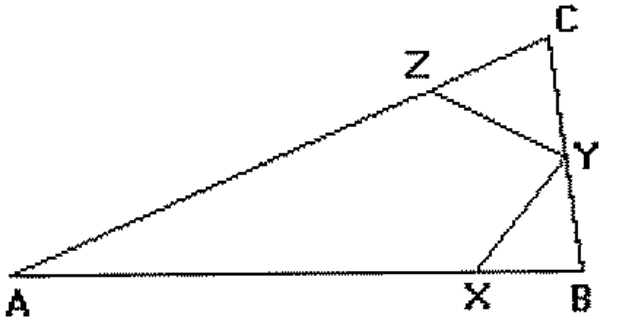
\includegraphics[width=.3\textwidth]{CONCURSO/EAM/IMAGES/2005/EAM200503IMG.png}
% \end{figure}


Na figura acima, \(AB = AC\), \(BX = BY\) e \(CZ = CY\). Se o ângulo \(A\) mede \(40^\circ\), quanto mede o ângulo \(XYZ\)?
    \begin{tasks}
        \task \(40^\circ\).
        \task \(50^\circ\).
        \task \(60^\circ\).
        \task \(70^\circ\).
        \task \(90^\circ\).
    \end{tasks}
\end{question}

\begin{question}%[codigo:EAM200504AMX; concurso:EAM; ano:2005; assunto:trigonometria no triângulo,trigonometria; alternativa:]

% \begin{figure}[h!]
    % 
    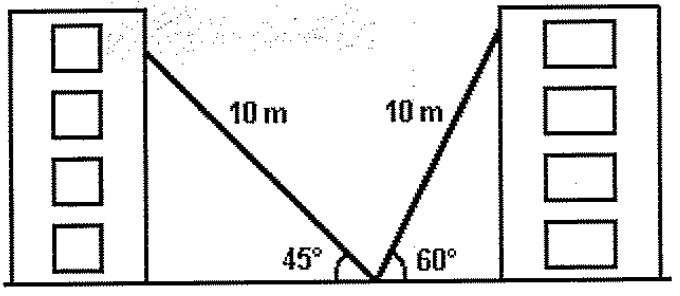
\includegraphics[width=.3\textwidth]{CONCURSO/EAM/IMAGES/2005/EAM200504IMG.png}
% \end{figure}

Uma escada de 10 metros de comprimento forma ângulo de \(60^\circ\) com a horizontal quando encostada ao edifício de um dos lados da rua, e ângulo de \(45^\circ\) se for encostada ao edifício do outro lado, apoiada no mesmo ponto do chão. A largura da rua, em metros, vale aproximadamente
    \begin{tasks}
        \task \(15\).
        \task \(14\).
        \task \(13\).
        \task \(12\).
        \task \(11\).
    \end{tasks}
\end{question}

\begin{question}%[codigo:EAM200505AMX; concurso:EAM; ano:2005; assunto:; alternativa:]
Uma balança assinala 325g para um certo copo cheio de água. Jogando-se metade da água fora, a balança passa a assinalar 180g. Para esse copo vazio, quanto tal balança assinalará em gramas?
    \begin{tasks}
        \task 20.
        \task 25.
        \task 35.
        \task 40.
        \task 45.
    \end{tasks}
\end{question}

\begin{question}%[codigo:EAM200506AMX; concurso:EAM; ano:2005; assunto:; alternativa:]
Numa competição de tiro-ao-alvo, cada atirador deve efetuar \(25\) disparos. Qual a porcentagem de acertos no alvo de um jogador que obtém \(+0,5\) pontos, sabendo-se que cada tiro no alvo vale \(+0,4\) e cada tiro fora do alvo vale \(-0,1\)?
    \begin{tasks}
        \task \(25\).
        \task \(24\).
        \task \(20\).
        \task \(16\).
        \task \(5\).
    \end{tasks}
\end{question}

\begin{question}%[codigo:EAM200507AMX; concurso:EAM; ano:2005; assunto:; alternativa:]
Um feirante compra duas unidades de maça por R\$ 0,75. Sabendo-se que ele vende o lote de seis maças por R\$ 3,00, quantas maças deverá vender para ter um lucro de R\$ 50,00?
    \begin{tasks}
        \task 50.
        \task 52.
        \task 400.
        \task 520.
        \task 600.
    \end{tasks}
\end{question}

\begin{question}%[codigo:EAM200508AMX; concurso:EAM; ano:2005; assunto:geometria,área de figuras; alternativa:]

% \begin{figure}[h!]
    
    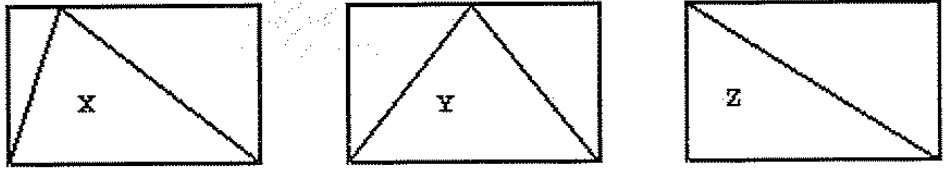
\includegraphics[width=.5\textwidth]{CONCURSO/EAM/IMAGES/2005/EAM200508IMG.png}
% \end{figure}

Considerando-se que, nas figuras acima, os triângulos \(X,Y\) e \(Z\) estejam inscritos em retângulos congruentes, pode-se afirmar que
    \begin{tasks}
        \task apenas as áreas dos triângulos \(X\) e \(Y\) são iguais.
        \task apenas as áreas dos triângulos \(X\) e \(Y\) são iguais.
        \task apenas as áreas dos triângulos \(Y\) e \(Z\) são iguais.
        \task as áreas dos triângulos \(X,Y\) e \(Z\) são iguais entre si.
        \task as áreas dos triângulos \(X, Y\) e Z são diferentes entre si.
    \end{tasks}
\end{question}

\begin{question}%[codigo:EAM200509AMX; concurso:EAM; ano:2005; assunto:múltiplos; alternativa:]
Numa unidade da Marinha, estão lotados: 200 terceiros sargentos; 160 segundos sargentos; e \(n\) primeiros sargentos. Se \(n\) representa \(2/5\) do número total de sargentos da referida unidade, pode-se afirmar que \(n\)
    \begin{tasks}
        \task é múltiplo de 15 e de 8.
        \task é múltiplo de 15 e não de 8.
        \task não é múltiplo de 15, nem de 8.
        \task não é múltiplo de 15, mas é múltiplo de 8.
        \task é múltiplo de 18.
    \end{tasks}
\end{question}

\begin{question}%[codigo:EAM200510AMX; concurso:EAM; ano:2005; assunto:; alternativa:]
Em uma sala retangular de piso plano nas dimensões 8,80m por 7,60m, deseja-se colocar lajotas quadradas iguais sem a necessidade de recortar qualquer peça. A medida máximo, em centímetros, do lado de cada lajota deverá ser igual a
    \begin{tasks}
        \task 10.
        \task 20.
        \task 30.
        \task 40.
        \task 50.
    \end{tasks}
\end{question}

\begin{question}%[codigo:EAM200511AMX; concurso:EAM; ano:2005; assunto:; alternativa:]
Fatorando-se a expressão \(ac + 2bc - ad -2bd\), obtém-se
    \begin{tasks}
        \task \((a+2b)(c-d)\).
        \task \((a-2b)(c-d)\).
        \task \((a-2b)(c+d)\).
        \task \((a+c)^2(a-d)\).
        \task \((a-c)(a+2b)\).
    \end{tasks}
\end{question}

\begin{question}%[codigo:EAM200512AMX; concurso:EAM; ano:2005; assunto:; alternativa:]
Caso seja cobrado um imposto de 5\% sobre o valor de qualquer saque efetuado em uma instituição financeira, qual será o saque máximo possível, em reais, a ser efetuado em uma conta cujo saldo é de 2 100,00 reais?
    \begin{tasks}
        \task 1 995,00.
        \task 2 000,00.
        \task 2 050,00.
        \task 2 075,00.
        \task 2 095,00.
    \end{tasks}
\end{question}

\begin{question}%[codigo:EAM200513AMX; concurso:EAM; ano:2005; assunto:volume; alternativa:]
A maquete de um reservatório \(R\), feita na escala \(1:500\), tem 8mm de largura, 10mm de comprimento e 8mm de altura. Qual é a capacidade em litros do reservatório \(R\)?
    \begin{tasks}
        \task 640.
        \task 800.
        \task 6400.
        \task 8000.
        \task 80000.
    \end{tasks}
\end{question}

\begin{question}%[codigo:EAM200514AMX; concurso:EAM; ano:2005; assunto:trângulo; alternativa:]
Em um triângulo, os lados medem 9cm, 12cm e 15cm. Quanto mede, em centímetros, a altura relativa ao maior lado desse triângulo?
    \begin{tasks}
        \task 8,0.
        \task 7,2.
        \task 6,0.
        \task 5,6.
        \task 4,3.
    \end{tasks}
\end{question}

\begin{question}%[codigo:EAM200515AMX; concurso:EAM; ano:2005; assunto:perímetro; alternativa:]

% \begin{figure}[h!]
    
    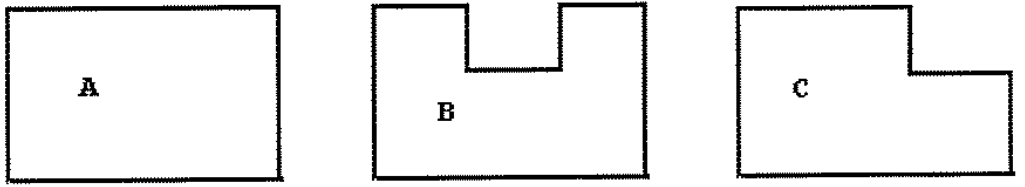
\includegraphics[width=.5\textwidth]{CONCURSO/EAM/IMAGES/2005/EAM200515IMG.png}
% \end{figure}

Considerando-se que a figura \(A\) seja um retângulo e as figuras \(B\) e \(C\) sejam obtidas, respectivamente, pela retirada da figura \(A\) de um quadrado de lado unitário, pode-se afirmar que
    \begin{tasks}
        \task apenas os perímetros das figuras \(A\) e \(B\) são iguais.
        \task apenas os perímetros das figuras \(A\) e \(C\) são iguais.
        \task apenas os perímetros das figuras \(B\) e \(C\) são iguais.
        \task os perímetros das figuras \(A,B\) e \(C\) são todos iguais.
        \task os perímetros das figuras \(A,B\) e \(C\) são todos diferentes.
    \end{tasks}
\end{question}

% \begin{question}%[codigo:EAM200600AMX; concurso:EAM; ano:2006; assunto:; alternativa:]

    \begin{tasks}
        \task 
        \task 
        \task 
        \task 
        \task 
    \end{tasks}
\end{question}

\begin{question}%[codigo:EAM200600AMX; concurso:EAM; ano:2006; assunto:; alternativa:]

    \begin{tasks}
        \task 
        \task 
        \task 
        \task 
        \task 
    \end{tasks}
\end{question}

\begin{question}%[codigo:EAM200600AMX; concurso:EAM; ano:2006; assunto:; alternativa:]

    \begin{tasks}
        \task 
        \task 
        \task 
        \task 
        \task 
    \end{tasks}
\end{question}

\begin{question}%[codigo:EAM200600AMX; concurso:EAM; ano:2006; assunto:; alternativa:]

    \begin{tasks}
        \task 
        \task 
        \task 
        \task 
        \task 
    \end{tasks}
\end{question}

\begin{question}%[codigo:EAM200600AMX; concurso:EAM; ano:2006; assunto:; alternativa:]

    \begin{tasks}
        \task 
        \task 
        \task 
        \task 
        \task 
    \end{tasks}
\end{question}

\begin{question}%[codigo:EAM200600AMX; concurso:EAM; ano:2006; assunto:; alternativa:]

    \begin{tasks}
        \task 
        \task 
        \task 
        \task 
        \task 
    \end{tasks}
\end{question}

\begin{question}%[codigo:EAM200600AMX; concurso:EAM; ano:2006; assunto:; alternativa:]

    \begin{tasks}
        \task 
        \task 
        \task 
        \task 
        \task 
    \end{tasks}
\end{question}

\begin{question}%[codigo:EAM200600AMX; concurso:EAM; ano:2006; assunto:; alternativa:]

    \begin{tasks}
        \task 
        \task 
        \task 
        \task 
        \task 
    \end{tasks}
\end{question}

\begin{question}%[codigo:EAM200600AMX; concurso:EAM; ano:2006; assunto:; alternativa:]

    \begin{tasks}
        \task 
        \task 
        \task 
        \task 
        \task 
    \end{tasks}
\end{question}

\begin{question}%[codigo:EAM200600AMX; concurso:EAM; ano:2006; assunto:; alternativa:]

    \begin{tasks}
        \task 
        \task 
        \task 
        \task 
        \task 
    \end{tasks}
\end{question}

\begin{question}%[codigo:EAM200600AMX; concurso:EAM; ano:2006; assunto:; alternativa:]

    \begin{tasks}
        \task 
        \task 
        \task 
        \task 
        \task 
    \end{tasks}
\end{question}

\begin{question}%[codigo:EAM200600AMX; concurso:EAM; ano:2006; assunto:; alternativa:]

    \begin{tasks}
        \task 
        \task 
        \task 
        \task 
        \task 
    \end{tasks}
\end{question}

\begin{question}%[codigo:EAM200600AMX; concurso:EAM; ano:2006; assunto:; alternativa:]

    \begin{tasks}
        \task 
        \task 
        \task 
        \task 
        \task 
    \end{tasks}
\end{question}

\begin{question}%[codigo:EAM200600AMX; concurso:EAM; ano:2006; assunto:; alternativa:]

    \begin{tasks}
        \task 
        \task 
        \task 
        \task 
        \task 
    \end{tasks}
\end{question}

\begin{question}%[codigo:EAM200600AMX; concurso:EAM; ano:2006; assunto:; alternativa:]

    \begin{tasks}
        \task 
        \task 
        \task 
        \task 
        \task 
    \end{tasks}
\end{question}

% \begin{question}%[codigo:EAM200700AMX; concurso:EAM; ano:2007; assunto:; alternativa:]

    \begin{tasks}
        \task 
        \task 
        \task 
        \task 
        \task 
    \end{tasks}
\end{question}

\begin{question}%[codigo:EAM200700AMX; concurso:EAM; ano:2007; assunto:; alternativa:]

    \begin{tasks}
        \task 
        \task 
        \task 
        \task 
        \task 
    \end{tasks}
\end{question}

\begin{question}%[codigo:EAM200700AMX; concurso:EAM; ano:2007; assunto:; alternativa:]

    \begin{tasks}
        \task 
        \task 
        \task 
        \task 
        \task 
    \end{tasks}
\end{question}

\begin{question}%[codigo:EAM200700AMX; concurso:EAM; ano:2007; assunto:; alternativa:]

    \begin{tasks}
        \task 
        \task 
        \task 
        \task 
        \task 
    \end{tasks}
\end{question}

\begin{question}%[codigo:EAM200700AMX; concurso:EAM; ano:2007; assunto:; alternativa:]

    \begin{tasks}
        \task 
        \task 
        \task 
        \task 
        \task 
    \end{tasks}
\end{question}

\begin{question}%[codigo:EAM200700AMX; concurso:EAM; ano:2007; assunto:; alternativa:]

    \begin{tasks}
        \task 
        \task 
        \task 
        \task 
        \task 
    \end{tasks}
\end{question}

\begin{question}%[codigo:EAM200700AMX; concurso:EAM; ano:2007; assunto:; alternativa:]

    \begin{tasks}
        \task 
        \task 
        \task 
        \task 
        \task 
    \end{tasks}
\end{question}

\begin{question}%[codigo:EAM200700AMX; concurso:EAM; ano:2007; assunto:; alternativa:]

    \begin{tasks}
        \task 
        \task 
        \task 
        \task 
        \task 
    \end{tasks}
\end{question}

\begin{question}%[codigo:EAM200700AMX; concurso:EAM; ano:2007; assunto:; alternativa:]

    \begin{tasks}
        \task 
        \task 
        \task 
        \task 
        \task 
    \end{tasks}
\end{question}

\begin{question}%[codigo:EAM200700AMX; concurso:EAM; ano:2007; assunto:; alternativa:]

    \begin{tasks}
        \task 
        \task 
        \task 
        \task 
        \task 
    \end{tasks}
\end{question}

\begin{question}%[codigo:EAM200700AMX; concurso:EAM; ano:2007; assunto:; alternativa:]

    \begin{tasks}
        \task 
        \task 
        \task 
        \task 
        \task 
    \end{tasks}
\end{question}

\begin{question}%[codigo:EAM200700AMX; concurso:EAM; ano:2007; assunto:; alternativa:]

    \begin{tasks}
        \task 
        \task 
        \task 
        \task 
        \task 
    \end{tasks}
\end{question}

\begin{question}%[codigo:EAM200700AMX; concurso:EAM; ano:2007; assunto:; alternativa:]

    \begin{tasks}
        \task 
        \task 
        \task 
        \task 
        \task 
    \end{tasks}
\end{question}

\begin{question}%[codigo:EAM200700AMX; concurso:EAM; ano:2007; assunto:; alternativa:]

    \begin{tasks}
        \task 
        \task 
        \task 
        \task 
        \task 
    \end{tasks}
\end{question}

\begin{question}%[codigo:EAM200700AMX; concurso:EAM; ano:2007; assunto:; alternativa:]

    \begin{tasks}
        \task 
        \task 
        \task 
        \task 
        \task 
    \end{tasks}
\end{question}

% \begin{question}%[concurso:EAM; ano:2008; assunto:; alternativa:]

    \begin{tasks}
        \task 
        \task 
        \task 
        \task 
        \task 
    \end{tasks}
\end{question}

\begin{question}%[concurso:EAM; ano:2008; assunto:; alternativa:]

    \begin{tasks}
        \task 
        \task 
        \task 
        \task 
        \task 
    \end{tasks}
\end{question}

\begin{question}%[concurso:EAM; ano:2008; assunto:; alternativa:]

    \begin{tasks}
        \task 
        \task 
        \task 
        \task 
        \task 
    \end{tasks}
\end{question}

\begin{question}%[concurso:EAM; ano:2008; assunto:; alternativa:]

    \begin{tasks}
        \task 
        \task 
        \task 
        \task 
        \task 
    \end{tasks}
\end{question}

\begin{question}%[concurso:EAM; ano:2008; assunto:; alternativa:]

    \begin{tasks}
        \task 
        \task 
        \task 
        \task 
        \task 
    \end{tasks}
\end{question}

\begin{question}%[concurso:EAM; ano:2008; assunto:; alternativa:]

    \begin{tasks}
        \task 
        \task 
        \task 
        \task 
        \task 
    \end{tasks}
\end{question}

\begin{question}%[concurso:EAM; ano:2008; assunto:; alternativa:]

    \begin{tasks}
        \task 
        \task 
        \task 
        \task 
        \task 
    \end{tasks}
\end{question}

\begin{question}%[concurso:EAM; ano:2008; assunto:; alternativa:]

    \begin{tasks}
        \task 
        \task 
        \task 
        \task 
        \task 
    \end{tasks}
\end{question}

\begin{question}%[concurso:EAM; ano:2008; assunto:; alternativa:]

    \begin{tasks}
        \task 
        \task 
        \task 
        \task 
        \task 
    \end{tasks}
\end{question}

\begin{question}%[concurso:EAM; ano:2008; assunto:; alternativa:]

    \begin{tasks}
        \task 
        \task 
        \task 
        \task 
        \task 
    \end{tasks}
\end{question}

\begin{question}%[concurso:EAM; ano:2008; assunto:; alternativa:]

    \begin{tasks}
        \task 
        \task 
        \task 
        \task 
        \task 
    \end{tasks}
\end{question}

\begin{question}%[concurso:EAM; ano:2008; assunto:; alternativa:]

    \begin{tasks}
        \task 
        \task 
        \task 
        \task 
        \task 
    \end{tasks}
\end{question}

\begin{question}%[concurso:EAM; ano:2008; assunto:; alternativa:]

    \begin{tasks}
        \task 
        \task 
        \task 
        \task 
        \task 
    \end{tasks}
\end{question}

\begin{question}%[concurso:EAM; ano:2008; assunto:; alternativa:]

    \begin{tasks}
        \task 
        \task 
        \task 
        \task 
        \task 
    \end{tasks}
\end{question}

\begin{question}%[concurso:EAM; ano:2008; assunto:; alternativa:]

    \begin{tasks}
        \task 
        \task 
        \task 
        \task 
        \task 
    \end{tasks}
\end{question}

% \begin{question}%[codigo:EAM200900AMX; concurso:EAM; ano:2009; assunto:; alternativa:]

    \begin{tasks}
        \task 
        \task 
        \task 
        \task 
        \task 
    \end{tasks}
\end{question}

\begin{question}%[codigo:EAM200900AMX; concurso:EAM; ano:2009; assunto:; alternativa:]

    \begin{tasks}
        \task 
        \task 
        \task 
        \task 
        \task 
    \end{tasks}
\end{question}

\begin{question}%[codigo:EAM200900AMX; concurso:EAM; ano:2009; assunto:; alternativa:]

    \begin{tasks}
        \task 
        \task 
        \task 
        \task 
        \task 
    \end{tasks}
\end{question}

\begin{question}%[codigo:EAM200900AMX; concurso:EAM; ano:2009; assunto:; alternativa:]

    \begin{tasks}
        \task 
        \task 
        \task 
        \task 
        \task 
    \end{tasks}
\end{question}

\begin{question}%[codigo:EAM200900AMX; concurso:EAM; ano:2009; assunto:; alternativa:]

    \begin{tasks}
        \task 
        \task 
        \task 
        \task 
        \task 
    \end{tasks}
\end{question}

\begin{question}%[codigo:EAM200900AMX; concurso:EAM; ano:2009; assunto:; alternativa:]

    \begin{tasks}
        \task 
        \task 
        \task 
        \task 
        \task 
    \end{tasks}
\end{question}

\begin{question}%[codigo:EAM200900AMX; concurso:EAM; ano:2009; assunto:; alternativa:]

    \begin{tasks}
        \task 
        \task 
        \task 
        \task 
        \task 
    \end{tasks}
\end{question}

\begin{question}%[codigo:EAM200900AMX; concurso:EAM; ano:2009; assunto:; alternativa:]

    \begin{tasks}
        \task 
        \task 
        \task 
        \task 
        \task 
    \end{tasks}
\end{question}

\begin{question}%[codigo:EAM200900AMX; concurso:EAM; ano:2009; assunto:; alternativa:]

    \begin{tasks}
        \task 
        \task 
        \task 
        \task 
        \task 
    \end{tasks}
\end{question}

\begin{question}%[codigo:EAM200900AMX; concurso:EAM; ano:2009; assunto:; alternativa:]

    \begin{tasks}
        \task 
        \task 
        \task 
        \task 
        \task 
    \end{tasks}
\end{question}

\begin{question}%[codigo:EAM200900AMX; concurso:EAM; ano:2009; assunto:; alternativa:]

    \begin{tasks}
        \task 
        \task 
        \task 
        \task 
        \task 
    \end{tasks}
\end{question}

\begin{question}%[codigo:EAM200900AMX; concurso:EAM; ano:2009; assunto:; alternativa:]

    \begin{tasks}
        \task 
        \task 
        \task 
        \task 
        \task 
    \end{tasks}
\end{question}

\begin{question}%[codigo:EAM200900AMX; concurso:EAM; ano:2009; assunto:; alternativa:]

    \begin{tasks}
        \task 
        \task 
        \task 
        \task 
        \task 
    \end{tasks}
\end{question}

\begin{question}%[codigo:EAM200900AMX; concurso:EAM; ano:2009; assunto:; alternativa:]

    \begin{tasks}
        \task 
        \task 
        \task 
        \task 
        \task 
    \end{tasks}
\end{question}

\begin{question}%[codigo:EAM200900AMX; concurso:EAM; ano:2009; assunto:; alternativa:]

    \begin{tasks}
        \task 
        \task 
        \task 
        \task 
        \task 
    \end{tasks}
\end{question}

% \begin{question}%[codigo:EAM201000AMX; concurso:EAM; ano:2010; assunto:; alternativa:]

    \begin{tasks}
        \task 
        \task 
        \task 
        \task 
        \task 
    \end{tasks}
\end{question}

\begin{question}%[codigo:EAM201000AMX; concurso:EAM; ano:2010; assunto:; alternativa:]

    \begin{tasks}
        \task 
        \task 
        \task 
        \task 
        \task 
    \end{tasks}
\end{question}

\begin{question}%[codigo:EAM201000AMX; concurso:EAM; ano:2010; assunto:; alternativa:]

    \begin{tasks}
        \task 
        \task 
        \task 
        \task 
        \task 
    \end{tasks}
\end{question}

\begin{question}%[codigo:EAM201000AMX; concurso:EAM; ano:2010; assunto:; alternativa:]

    \begin{tasks}
        \task 
        \task 
        \task 
        \task 
        \task 
    \end{tasks}
\end{question}

\begin{question}%[codigo:EAM201000AMX; concurso:EAM; ano:2010; assunto:; alternativa:]

    \begin{tasks}
        \task 
        \task 
        \task 
        \task 
        \task 
    \end{tasks}
\end{question}

\begin{question}%[codigo:EAM201000AMX; concurso:EAM; ano:2010; assunto:; alternativa:]

    \begin{tasks}
        \task 
        \task 
        \task 
        \task 
        \task 
    \end{tasks}
\end{question}

\begin{question}%[codigo:EAM201000AMX; concurso:EAM; ano:2010; assunto:; alternativa:]

    \begin{tasks}
        \task 
        \task 
        \task 
        \task 
        \task 
    \end{tasks}
\end{question}

\begin{question}%[codigo:EAM201000AMX; concurso:EAM; ano:2010; assunto:; alternativa:]

    \begin{tasks}
        \task 
        \task 
        \task 
        \task 
        \task 
    \end{tasks}
\end{question}

\begin{question}%[codigo:EAM201000AMX; concurso:EAM; ano:2010; assunto:; alternativa:]

    \begin{tasks}
        \task 
        \task 
        \task 
        \task 
        \task 
    \end{tasks}
\end{question}

\begin{question}%[codigo:EAM201000AMX; concurso:EAM; ano:2010; assunto:; alternativa:]

    \begin{tasks}
        \task 
        \task 
        \task 
        \task 
        \task 
    \end{tasks}
\end{question}

\begin{question}%[codigo:EAM201000AMX; concurso:EAM; ano:2010; assunto:; alternativa:]

    \begin{tasks}
        \task 
        \task 
        \task 
        \task 
        \task 
    \end{tasks}
\end{question}

\begin{question}%[codigo:EAM201000AMX; concurso:EAM; ano:2010; assunto:; alternativa:]

    \begin{tasks}
        \task 
        \task 
        \task 
        \task 
        \task 
    \end{tasks}
\end{question}

\begin{question}%[codigo:EAM201000AMX; concurso:EAM; ano:2010; assunto:; alternativa:]

    \begin{tasks}
        \task 
        \task 
        \task 
        \task 
        \task 
    \end{tasks}
\end{question}

\begin{question}%[codigo:EAM201000AMX; concurso:EAM; ano:2010; assunto:; alternativa:]

    \begin{tasks}
        \task 
        \task 
        \task 
        \task 
        \task 
    \end{tasks}
\end{question}

\begin{question}%[codigo:EAM201000AMX; concurso:EAM; ano:2010; assunto:; alternativa:]

    \begin{tasks}
        \task 
        \task 
        \task 
        \task 
        \task 
    \end{tasks}
\end{question}

% \begin{question}%[concurso:EAM; ano:2011; assunto:; alternativa:]

    \begin{tasks}
        \task 
        \task 
        \task 
        \task 
        \task 
    \end{tasks}
\end{question}

\begin{question}%[concurso:EAM; ano:2011; assunto:; alternativa:]

    \begin{tasks}
        \task 
        \task 
        \task 
        \task 
        \task 
    \end{tasks}
\end{question}

\begin{question}%[concurso:EAM; ano:2011; assunto:; alternativa:]

    \begin{tasks}
        \task 
        \task 
        \task 
        \task 
        \task 
    \end{tasks}
\end{question}

\begin{question}%[concurso:EAM; ano:2011; assunto:; alternativa:]

    \begin{tasks}
        \task 
        \task 
        \task 
        \task 
        \task 
    \end{tasks}
\end{question}

\begin{question}%[concurso:EAM; ano:2011; assunto:; alternativa:]

    \begin{tasks}
        \task 
        \task 
        \task 
        \task 
        \task 
    \end{tasks}
\end{question}

\begin{question}%[concurso:EAM; ano:2011; assunto:; alternativa:]

    \begin{tasks}
        \task 
        \task 
        \task 
        \task 
        \task 
    \end{tasks}
\end{question}

\begin{question}%[concurso:EAM; ano:2011; assunto:; alternativa:]

    \begin{tasks}
        \task 
        \task 
        \task 
        \task 
        \task 
    \end{tasks}
\end{question}

\begin{question}%[concurso:EAM; ano:2011; assunto:; alternativa:]

    \begin{tasks}
        \task 
        \task 
        \task 
        \task 
        \task 
    \end{tasks}
\end{question}

\begin{question}%[concurso:EAM; ano:2011; assunto:; alternativa:]

    \begin{tasks}
        \task 
        \task 
        \task 
        \task 
        \task 
    \end{tasks}
\end{question}

\begin{question}%[concurso:EAM; ano:2011; assunto:; alternativa:]

    \begin{tasks}
        \task 
        \task 
        \task 
        \task 
        \task 
    \end{tasks}
\end{question}

\begin{question}%[concurso:EAM; ano:2011; assunto:; alternativa:]

    \begin{tasks}
        \task 
        \task 
        \task 
        \task 
        \task 
    \end{tasks}
\end{question}

\begin{question}%[concurso:EAM; ano:2011; assunto:; alternativa:]

    \begin{tasks}
        \task 
        \task 
        \task 
        \task 
        \task 
    \end{tasks}
\end{question}

\begin{question}%[concurso:EAM; ano:2011; assunto:; alternativa:]

    \begin{tasks}
        \task 
        \task 
        \task 
        \task 
        \task 
    \end{tasks}
\end{question}

\begin{question}%[concurso:EAM; ano:2011; assunto:; alternativa:]

    \begin{tasks}
        \task 
        \task 
        \task 
        \task 
        \task 
    \end{tasks}
\end{question}

\begin{question}%[concurso:EAM; ano:2011; assunto:; alternativa:]

    \begin{tasks}
        \task 
        \task 
        \task 
        \task 
        \task 
    \end{tasks}
\end{question}

% \begin{question}%[concurso:EAM; ano:2012; assunto:; alternativa:]

    \begin{tasks}
        \task 
        \task 
        \task 
        \task 
        \task 
    \end{tasks}
\end{question}

\begin{question}%[concurso:EAM; ano:2012; assunto:; alternativa:]

    \begin{tasks}
        \task 
        \task 
        \task 
        \task 
        \task 
    \end{tasks}
\end{question}

\begin{question}%[concurso:EAM; ano:2012; assunto:; alternativa:]

    \begin{tasks}
        \task 
        \task 
        \task 
        \task 
        \task 
    \end{tasks}
\end{question}

\begin{question}%[concurso:EAM; ano:2012; assunto:; alternativa:]

    \begin{tasks}
        \task 
        \task 
        \task 
        \task 
        \task 
    \end{tasks}
\end{question}

\begin{question}%[concurso:EAM; ano:2012; assunto:; alternativa:]

    \begin{tasks}
        \task 
        \task 
        \task 
        \task 
        \task 
    \end{tasks}
\end{question}

\begin{question}%[concurso:EAM; ano:2012; assunto:; alternativa:]

    \begin{tasks}
        \task 
        \task 
        \task 
        \task 
        \task 
    \end{tasks}
\end{question}

\begin{question}%[concurso:EAM; ano:2012; assunto:; alternativa:]

    \begin{tasks}
        \task 
        \task 
        \task 
        \task 
        \task 
    \end{tasks}
\end{question}

\begin{question}%[concurso:EAM; ano:2012; assunto:; alternativa:]

    \begin{tasks}
        \task 
        \task 
        \task 
        \task 
        \task 
    \end{tasks}
\end{question}

\begin{question}%[concurso:EAM; ano:2012; assunto:; alternativa:]

    \begin{tasks}
        \task 
        \task 
        \task 
        \task 
        \task 
    \end{tasks}
\end{question}

\begin{question}%[concurso:EAM; ano:2012; assunto:; alternativa:]

    \begin{tasks}
        \task 
        \task 
        \task 
        \task 
        \task 
    \end{tasks}
\end{question}

\begin{question}%[concurso:EAM; ano:2012; assunto:; alternativa:]

    \begin{tasks}
        \task 
        \task 
        \task 
        \task 
        \task 
    \end{tasks}
\end{question}

\begin{question}%[concurso:EAM; ano:2012; assunto:; alternativa:]

    \begin{tasks}
        \task 
        \task 
        \task 
        \task 
        \task 
    \end{tasks}
\end{question}

\begin{question}%[concurso:EAM; ano:2012; assunto:; alternativa:]

    \begin{tasks}
        \task 
        \task 
        \task 
        \task 
        \task 
    \end{tasks}
\end{question}

\begin{question}%[concurso:EAM; ano:2012; assunto:; alternativa:]

    \begin{tasks}
        \task 
        \task 
        \task 
        \task 
        \task 
    \end{tasks}
\end{question}

\begin{question}%[concurso:EAM; ano:2012; assunto:; alternativa:]

    \begin{tasks}
        \task 
        \task 
        \task 
        \task 
        \task 
    \end{tasks}
\end{question}

% \begin{question}%[codigo:EAM201300AMX; concurso:EAM; ano:2013; assunto:; alternativa:]

    \begin{tasks}
        \task 
        \task 
        \task 
        \task 
        \task 
    \end{tasks}
\end{question}

\begin{question}%[codigo:EAM201300AMX; concurso:EAM; ano:2013; assunto:; alternativa:]

    \begin{tasks}
        \task 
        \task 
        \task 
        \task 
        \task 
    \end{tasks}
\end{question}

\begin{question}%[codigo:EAM201300AMX; concurso:EAM; ano:2013; assunto:; alternativa:]

    \begin{tasks}
        \task 
        \task 
        \task 
        \task 
        \task 
    \end{tasks}
\end{question}

\begin{question}%[codigo:EAM201300AMX; concurso:EAM; ano:2013; assunto:; alternativa:]

    \begin{tasks}
        \task 
        \task 
        \task 
        \task 
        \task 
    \end{tasks}
\end{question}

\begin{question}%[codigo:EAM201300AMX; concurso:EAM; ano:2013; assunto:; alternativa:]

    \begin{tasks}
        \task 
        \task 
        \task 
        \task 
        \task 
    \end{tasks}
\end{question}

\begin{question}%[codigo:EAM201300AMX; concurso:EAM; ano:2013; assunto:; alternativa:]

    \begin{tasks}
        \task 
        \task 
        \task 
        \task 
        \task 
    \end{tasks}
\end{question}

\begin{question}%[codigo:EAM201300AMX; concurso:EAM; ano:2013; assunto:; alternativa:]

    \begin{tasks}
        \task 
        \task 
        \task 
        \task 
        \task 
    \end{tasks}
\end{question}

\begin{question}%[codigo:EAM201300AMX; concurso:EAM; ano:2013; assunto:; alternativa:]

    \begin{tasks}
        \task 
        \task 
        \task 
        \task 
        \task 
    \end{tasks}
\end{question}

\begin{question}%[codigo:EAM201300AMX; concurso:EAM; ano:2013; assunto:; alternativa:]

    \begin{tasks}
        \task 
        \task 
        \task 
        \task 
        \task 
    \end{tasks}
\end{question}

\begin{question}%[codigo:EAM201300AMX; concurso:EAM; ano:2013; assunto:; alternativa:]

    \begin{tasks}
        \task 
        \task 
        \task 
        \task 
        \task 
    \end{tasks}
\end{question}

\begin{question}%[codigo:EAM201300AMX; concurso:EAM; ano:2013; assunto:; alternativa:]

    \begin{tasks}
        \task 
        \task 
        \task 
        \task 
        \task 
    \end{tasks}
\end{question}

\begin{question}%[codigo:EAM201300AMX; concurso:EAM; ano:2013; assunto:; alternativa:]

    \begin{tasks}
        \task 
        \task 
        \task 
        \task 
        \task 
    \end{tasks}
\end{question}

\begin{question}%[codigo:EAM201300AMX; concurso:EAM; ano:2013; assunto:; alternativa:]

    \begin{tasks}
        \task 
        \task 
        \task 
        \task 
        \task 
    \end{tasks}
\end{question}

\begin{question}%[codigo:EAM201300AMX; concurso:EAM; ano:2013; assunto:; alternativa:]

    \begin{tasks}
        \task 
        \task 
        \task 
        \task 
        \task 
    \end{tasks}
\end{question}

\begin{question}%[codigo:EAM201300AMX; concurso:EAM; ano:2013; assunto:; alternativa:]

    \begin{tasks}
        \task 
        \task 
        \task 
        \task 
        \task 
    \end{tasks}
\end{question}

% \begin{question}%[concurso:EAM; ano:2014; assunto:; alternativa:]

    \begin{tasks}
        \task 
        \task 
        \task 
        \task 
        \task 
    \end{tasks}
\end{question}

\begin{question}%[concurso:EAM; ano:2014; assunto:; alternativa:]

    \begin{tasks}
        \task 
        \task 
        \task 
        \task 
        \task 
    \end{tasks}
\end{question}

\begin{question}%[concurso:EAM; ano:2014; assunto:; alternativa:]

    \begin{tasks}
        \task 
        \task 
        \task 
        \task 
        \task 
    \end{tasks}
\end{question}

\begin{question}%[concurso:EAM; ano:2014; assunto:; alternativa:]

    \begin{tasks}
        \task 
        \task 
        \task 
        \task 
        \task 
    \end{tasks}
\end{question}

\begin{question}%[concurso:EAM; ano:2014; assunto:; alternativa:]

    \begin{tasks}
        \task 
        \task 
        \task 
        \task 
        \task 
    \end{tasks}
\end{question}

\begin{question}%[concurso:EAM; ano:2014; assunto:; alternativa:]

    \begin{tasks}
        \task 
        \task 
        \task 
        \task 
        \task 
    \end{tasks}
\end{question}

\begin{question}%[concurso:EAM; ano:2014; assunto:; alternativa:]

    \begin{tasks}
        \task 
        \task 
        \task 
        \task 
        \task 
    \end{tasks}
\end{question}

\begin{question}%[concurso:EAM; ano:2014; assunto:; alternativa:]

    \begin{tasks}
        \task 
        \task 
        \task 
        \task 
        \task 
    \end{tasks}
\end{question}

\begin{question}%[concurso:EAM; ano:2014; assunto:; alternativa:]

    \begin{tasks}
        \task 
        \task 
        \task 
        \task 
        \task 
    \end{tasks}
\end{question}

\begin{question}%[concurso:EAM; ano:2014; assunto:; alternativa:]

    \begin{tasks}
        \task 
        \task 
        \task 
        \task 
        \task 
    \end{tasks}
\end{question}

\begin{question}%[concurso:EAM; ano:2014; assunto:; alternativa:]

    \begin{tasks}
        \task 
        \task 
        \task 
        \task 
        \task 
    \end{tasks}
\end{question}

\begin{question}%[concurso:EAM; ano:2014; assunto:; alternativa:]

    \begin{tasks}
        \task 
        \task 
        \task 
        \task 
        \task 
    \end{tasks}
\end{question}

\begin{question}%[concurso:EAM; ano:2014; assunto:; alternativa:]

    \begin{tasks}
        \task 
        \task 
        \task 
        \task 
        \task 
    \end{tasks}
\end{question}

\begin{question}%[concurso:EAM; ano:2014; assunto:; alternativa:]

    \begin{tasks}
        \task 
        \task 
        \task 
        \task 
        \task 
    \end{tasks}
\end{question}

\begin{question}%[concurso:EAM; ano:2014; assunto:; alternativa:]

    \begin{tasks}
        \task 
        \task 
        \task 
        \task 
        \task 
    \end{tasks}
\end{question}

% \begin{question}%[codigo:EAM201500AMX; concurso:EAM; ano:2015; assunto:; alternativa:]

    \begin{tasks}
        \task 
        \task 
        \task 
        \task 
        \task 
    \end{tasks}
\end{question}

\begin{question}%[codigo:EAM201500AMX; concurso:EAM; ano:2015; assunto:; alternativa:]

    \begin{tasks}
        \task 
        \task 
        \task 
        \task 
        \task 
    \end{tasks}
\end{question}

\begin{question}%[codigo:EAM201500AMX; concurso:EAM; ano:2015; assunto:; alternativa:]

    \begin{tasks}
        \task 
        \task 
        \task 
        \task 
        \task 
    \end{tasks}
\end{question}

\begin{question}%[codigo:EAM201500AMX; concurso:EAM; ano:2015; assunto:; alternativa:]

    \begin{tasks}
        \task 
        \task 
        \task 
        \task 
        \task 
    \end{tasks}
\end{question}

\begin{question}%[codigo:EAM201500AMX; concurso:EAM; ano:2015; assunto:; alternativa:]

    \begin{tasks}
        \task 
        \task 
        \task 
        \task 
        \task 
    \end{tasks}
\end{question}

\begin{question}%[codigo:EAM201500AMX; concurso:EAM; ano:2015; assunto:; alternativa:]

    \begin{tasks}
        \task 
        \task 
        \task 
        \task 
        \task 
    \end{tasks}
\end{question}

\begin{question}%[codigo:EAM201500AMX; concurso:EAM; ano:2015; assunto:; alternativa:]

    \begin{tasks}
        \task 
        \task 
        \task 
        \task 
        \task 
    \end{tasks}
\end{question}

\begin{question}%[codigo:EAM201500AMX; concurso:EAM; ano:2015; assunto:; alternativa:]

    \begin{tasks}
        \task 
        \task 
        \task 
        \task 
        \task 
    \end{tasks}
\end{question}

\begin{question}%[codigo:EAM201500AMX; concurso:EAM; ano:2015; assunto:; alternativa:]

    \begin{tasks}
        \task 
        \task 
        \task 
        \task 
        \task 
    \end{tasks}
\end{question}

\begin{question}%[codigo:EAM201500AMX; concurso:EAM; ano:2015; assunto:; alternativa:]

    \begin{tasks}
        \task 
        \task 
        \task 
        \task 
        \task 
    \end{tasks}
\end{question}

\begin{question}%[codigo:EAM201500AMX; concurso:EAM; ano:2015; assunto:; alternativa:]

    \begin{tasks}
        \task 
        \task 
        \task 
        \task 
        \task 
    \end{tasks}
\end{question}

\begin{question}%[codigo:EAM201500AMX; concurso:EAM; ano:2015; assunto:; alternativa:]

    \begin{tasks}
        \task 
        \task 
        \task 
        \task 
        \task 
    \end{tasks}
\end{question}

\begin{question}%[codigo:EAM201500AMX; concurso:EAM; ano:2015; assunto:; alternativa:]

    \begin{tasks}
        \task 
        \task 
        \task 
        \task 
        \task 
    \end{tasks}
\end{question}

\begin{question}%[codigo:EAM201500AMX; concurso:EAM; ano:2015; assunto:; alternativa:]

    \begin{tasks}
        \task 
        \task 
        \task 
        \task 
        \task 
    \end{tasks}
\end{question}

\begin{question}%[codigo:EAM201500AMX; concurso:EAM; ano:2015; assunto:; alternativa:]

    \begin{tasks}
        \task 
        \task 
        \task 
        \task 
        \task 
    \end{tasks}
\end{question}

% \begin{question}%[codigo:%[codigo:EAM202201AMX; concurso:EAM;AMX; concurso:EAM; ano:2016; assunto:; alternativa:]

    \begin{tasks}
        \task 
        \task 
        \task 
        \task 
        \task 
    \end{tasks}
\end{question}

\begin{question}%[codigo:EAM201600AMX; concurso:EAM; ano:2016; assunto:; alternativa:]

    \begin{tasks}
        \task 
        \task 
        \task 
        \task 
        \task 
    \end{tasks}
\end{question}

\begin{question}%[codigo:EAM201600AMX; concurso:EAM; ano:2016; assunto:; alternativa:]

    \begin{tasks}
        \task 
        \task 
        \task 
        \task 
        \task 
    \end{tasks}
\end{question}

\begin{question}%[codigo:EAM201600AMX; concurso:EAM; ano:2016; assunto:; alternativa:]

    \begin{tasks}
        \task 
        \task 
        \task 
        \task 
        \task 
    \end{tasks}
\end{question}

\begin{question}%[codigo:EAM201600AMX; concurso:EAM; ano:2016; assunto:; alternativa:]

    \begin{tasks}
        \task 
        \task 
        \task 
        \task 
        \task 
    \end{tasks}
\end{question}

\begin{question}%[codigo:EAM201600AMX; concurso:EAM; ano:2016; assunto:; alternativa:]

    \begin{tasks}
        \task 
        \task 
        \task 
        \task 
        \task 
    \end{tasks}
\end{question}

\begin{question}%[codigo:EAM201600AMX; concurso:EAM; ano:2016; assunto:; alternativa:]

    \begin{tasks}
        \task 
        \task 
        \task 
        \task 
        \task 
    \end{tasks}
\end{question}

\begin{question}%[codigo:EAM201600AMX; concurso:EAM; ano:2016; assunto:; alternativa:]

    \begin{tasks}
        \task 
        \task 
        \task 
        \task 
        \task 
    \end{tasks}
\end{question}

\begin{question}%[codigo:EAM201600AMX; concurso:EAM; ano:2016; assunto:; alternativa:]

    \begin{tasks}
        \task 
        \task 
        \task 
        \task 
        \task 
    \end{tasks}
\end{question}

\begin{question}%[codigo:EAM201600AMX; concurso:EAM; ano:2016; assunto:; alternativa:]

    \begin{tasks}
        \task 
        \task 
        \task 
        \task 
        \task 
    \end{tasks}
\end{question}

\begin{question}%[codigo:EAM201600AMX; concurso:EAM; ano:2016; assunto:; alternativa:]

    \begin{tasks}
        \task 
        \task 
        \task 
        \task 
        \task 
    \end{tasks}
\end{question}

\begin{question}%[codigo:EAM201600AMX; concurso:EAM; ano:2016; assunto:; alternativa:]

    \begin{tasks}
        \task 
        \task 
        \task 
        \task 
        \task 
    \end{tasks}
\end{question}

\begin{question}%[codigo:EAM201600AMX; concurso:EAM; ano:2016; assunto:; alternativa:]

    \begin{tasks}
        \task 
        \task 
        \task 
        \task 
        \task 
    \end{tasks}
\end{question}

\begin{question}%[codigo:EAM201600AMX; concurso:EAM; ano:2016; assunto:; alternativa:]

    \begin{tasks}
        \task 
        \task 
        \task 
        \task 
        \task 
    \end{tasks}
\end{question}

\begin{question}%[codigo:EAM201600AMX; concurso:EAM; ano:2016; assunto:; alternativa:]

    \begin{tasks}
        \task 
        \task 
        \task 
        \task 
        \task 
    \end{tasks}
\end{question}

% \begin{question}%[codigo:EAM201701AMX; concurso:EAM; ano:2017; assunto:; alternativa:]
Sendo \(x - \frac{2}{x} = a\), então \(x^2 + \frac{4}{x}\) é igual a:
    \begin{tasks}
        \task \(a^2 + 4\).
        \task \(a^2 - 4\).
        \task \(a^2\).
        \task \(a + 4\).
        \task \(a - 4\).
    \end{tasks}
\end{question}

\begin{question}%[codigo:EAM201702AMX; concurso:EAM; ano:2017; assunto:; alternativa:]
Analise a figura a seguir.

INSERIR FIGURA

Calcule a soma das áreas hachuradas da figura acima, sabendo que os polígonos I e II são quadrados, e assinale a opção correta.
    \begin{tasks}
        \task \(22\sqrt{3}\).
        \task \(22\).
        \task \(13 + 4\sqrt{3}\).
        \task \(11\).
        \task \(11\sqrt{3}\).
    \end{tasks}
\end{question}

\begin{question}%[codigo:EAM201703AMX; concurso:EAM; ano:2017; assunto:; alternativa:]
Observe a figura a seguir.

INSERIR FIGURA

Sabendo que, na figura acima, as reatas \(r\) e \(s\) são paralelas, é correto afirmar que o valor de \(x\) é igual a:
    \begin{tasks}
        \task 90\(^\circ\).
        \task 85\(^\circ\).
        \task 80\(^\circ\).
        \task 75\(^\circ\).
        \task 70\(^\circ\).
    \end{tasks}
\end{question}

\begin{question}%[codigo:EAM201704AMX; concurso:EAM; ano:2017; assunto:; alternativa:]
Deseja-se azulejar, até o teto, as 4 paredes de uma cozinha. Sabe-se que a cozinha possui 2 portas medindo 210cm de altura e 80cm de largura cada uma, e uma janela com 150cm de altura e 110cm de comprimento. O comprimento, a largura e a altura da cozinha são iguais a 5,0m, 4,0m e 3,0m, respectivamente. Determine o número mínimo de metros quadrados inteiros de azulejos que devem ser comprados a assinale a opção correta.
    \begin{tasks}
        \task 42.
        \task 43.
        \task 49.
        \task 55.
        \task 58.
    \end{tasks}
\end{question}

\begin{question}%[codigo:EAM201705AMX; concurso:EAM; ano:2017; assunto:; alternativa:]
Considerando \(n(P)\) como a notação que determina o número de elementos de um conjunto \(P,A \times X\) como o produto cartesiano entre dois conjuntos finitos A e B e sabendo-se ainda que \(n(A) = 2x - 3, n(B) = x-5\) e \(n(A \times B)= x^2 +10x -27\), é correto afirmar que o valor numérico de \(x\) é:
    \begin{tasks}
        \task um número primo.
        \task um múltiplo de 5.
        \task um múltiplo de 7.
        \task um múltiplo de 11.
        \task um múltiplo de 13.
    \end{tasks}
\end{question}

\begin{question}%[codigo:EAM201706AMX; concurso:EAM; ano:2017; assunto:; alternativa:]
Seja a função real \(f\) definida por \(f(x) = \frac{x+k}{p}\). Sabendo-se que \(f(3) = 2\) e \(f(5) = 4\), determine o valor de \(k+p\) e assinale a opção correta.
    \begin{tasks}
        \task 0.
        \task 1.
        \task 2.
        \task 3.
        \task 4.
    \end{tasks}
\end{question}

\begin{question}%[codigo:EAM201707AMX; concurso:EAM; ano:2017; assunto:; alternativa:]
Sabendo-se que \(A\) e \(B\) são subconjuntos finitos de \(U\), que \( \bar{A}\) é a notação para a operação complementar de \(A\) em relação a \(U\), que \(\bar{A} = \{q,r,s,t,u\}, A \cap B = \{o,p\}\) e \(A \cup B = \{m,n,o,p,q,r\}\), é correto afirmar que:
    \begin{tasks}
        \task \(A\) tem dois elementos e \(B\) tem quatro elementos.
        \task \(A\) tem quatro elementos e \(B\) tem dois elementos.
        \task \(A\) tem três elementos e \(B\) tem três elementos.
        \task \(A\) tem quatro elementos e \(B\) tem quatro elementos.
        \task \(A\) tem um elemento e \(B\) tem cinco elementos.
    \end{tasks}
\end{question}

\begin{question}%[codigo:EAM201708AMX; concurso:EAM; ano:2017; assunto:; alternativa:]
Sabendo que a fração \(\frac{y}{4}\) é proporcional à fração \(\frac{3}{6-2\sqrt{3}}\), é correto afirmar que \(y\) é igual a:
    \begin{tasks}
        \task \( 1 - 2\sqrt{3}\).
        \task \( 6 + 3\sqrt{3}\).
        \task \( 2 - \sqrt{3}\).
        \task \( 4 + 3\sqrt{3}\).
        \task \( 3+ \sqrt{3}\).
    \end{tasks}
\end{question}

\begin{question}%[codigo:EAM201709AMX; concurso:EAM; ano:2017; assunto:; alternativa:]
A soma de um número \(x\) com o dobro de um número \(y\) é \(-7\); e a diferença entre o triplo desse número \(x\) e o número \(y\) é igual a \(7\). Sendo assim, é correto afirmar que o produto \(xy\) é igual a:
    \begin{tasks}
        \task -15.
        \task -12.
        \task -10.
        \task -4.
        \task -2.
    \end{tasks}
\end{question}

\begin{question}%[codigo:EAM201710AMX; concurso:EAM; ano:2017; assunto:; alternativa:]
O número natural \(N= 2^3 \cdot 3^p\) possui 20 divisores positivos. Sendo assim, o valor de \(p\) é:
    \begin{tasks}
        \task 2.
        \task 3.
        \task 4.
        \task 5.
        \task 6.
    \end{tasks}
\end{question}

\begin{question}%[codigo:EAM201711AMX; concurso:EAM; ano:2017; assunto:; alternativa:]
Apoiado em dois pilares construídos sobre um terreno plano e distantes 3m um do outro, constrói-se um telhado, cuja inclinação é de 30\(^\circ\) em relação ao piso. Se o pular de menor altura mede 4 metros, qual é a altura do outro pilar? Dado: \(\sqrt{3} = 1,7\)
    \begin{tasks}
        \task 5,5m.
        \task 5,7m.
        \task 6,0m.
        \task 6,5m.
        \task 6,9m.
    \end{tasks}
\end{question}

\begin{question}%[codigo:EAM201712AMX; concurso:EAM; ano:2017; assunto:; alternativa:]
Um colecionador de selos criou um catálogo de selos em uma pasta com 20 páginas numeradas de 1 até 20, cada uma com 15 selos, distribuídos em 5 linhas e 3 colunas. Os selos foram numerados de 1 a 300. Nesse catálogo, alguns selos são considerados raros e ocupam as posições 9\textordfeminine{},18\textordfeminine{},27\textordfeminine{},36\textordfeminine{} e assim sucessivamente. Depois que o catálogo for completado com todos os selos, é correto afirmar que o número de última página que terminará com um selo raro será
    \begin{tasks}
        \task 9.
        \task 11.
        \task 12.
        \task 18.
        \task 20.
    \end{tasks}
\end{question}

\begin{question}%[codigo:EAM201713AMX; concurso:EAM; ano:2017; assunto:; alternativa:]
No dia 17-10-2016, á zero hora, iniciou-se mais uma vez o horário de verão no Rio de Janeiro, que tem sido usado com objetivo de economizar energia elétrica nos momentos de pico e evitar sobrecarga no sistema. No dia 16-10-2016, um avião partiu de St. John's, Canadá, com destino ao Rio de Janeiro. A saída aconteceu às 21h e 45min e o voo teve duração de 13h e 45min. Considerando que entre St. John's e Rio de Janeiro não há diferença de fuso horário, a que horas local o avião chegou ao Rio de Janeiro?
    \begin{tasks}
        \task 9h e 30min.
        \task 10h e 30min.
        \task 11h e 15min.
        \task 11h e 45min.
        \task 12h e 30min.
    \end{tasks}
\end{question}

\begin{question}%[codigo:EAM201714AMX; concurso:EAM; ano:2017; assunto:; alternativa:]
Observe a figura a seguir.

INSERIR IMAGEM

Na figura acima, tem-se um triângulo isósceles \(ACD\), no qual o segmento \(\overline{AB}\) mede 3cm, o lado desigual \(AD\) mede \(10\sqrt{2}\)cm e os segmentos \(\overline{AC}\) e \(\overline{CD}\) são perpendiculares. Sendo assim, é correto afirmar que o segmento \(\overline{BD}\) mede:
    \begin{tasks}
        \task \(\sqrt{53}\)cm.
        \task \(\sqrt{97}\)cm.
        \task \(\sqrt{111}\)cm.
        \task \(\sqrt{149}\)cm.
        \task \(\sqrt{161}\)cm.
    \end{tasks}
\end{question}

\begin{question}%[codigo:EAM201715AMX; concurso:EAM; ano:2017; assunto:; alternativa:]
A área de um retângulo corresponde à expressão \(K^2-10k-24\) quando \(k=36\). Sendo assim, calcule suas dimensões e assinale a opção correta.
    \begin{tasks}
        \task 38 e 24.
        \task 36 e 32.
        \task 63 e 24.
        \task 54 e 38.
        \task 32 e 24.
    \end{tasks}
\end{question}

\begin{question}%[codigo:EAM201716AMX; concurso:EAM; ano:2017; assunto:; alternativa:]
Observe a figura abaixo.

INSERIR FIGURA

Um prédio projeta no solo uma sombra de 30m de extensão no mesmo instante em que uma pessoa de 1,80m projeta uma sombra de 2,0m. Pode-se afirmar que a altura do prédio vale
    \begin{tasks}
        \task 27m.
        \task 30m.
        \task 33m.
        \task 36m.
        \task 40m.
    \end{tasks}
\end{question}
% \begin{question}%[concurso:EAM; ano:2018; assunto:; alternativa:]
A partir de um dos vértices de um polígono convexo pode-se traçar tantas diagonais quantas são o total de diagonais de um pentágono. É correto afirmar que esse polígono é um:
    \begin{tasks}
        \task Hexágono.
        \task Heptágono.
        \task Octógono.
        \task Decágono.
        \task Dodecágono.
    \end{tasks}
\end{question}

\begin{question}%[concurso:EAM; ano:2018; assunto:; alternativa:]
Considere a função \(f(x) = k \cos(x)\), onde \(K\) é uma constante real, diferente de zero, e \(x\) é valor de graus. É correto afirmar que a razão entre \(f(60^\circ)\) e \(f(45^\circ)\) é igual a:
    \begin{tasks}
        \task \(\frac{\sqrt{2}}{2}\).
        \task \(\frac{1}{2}\).
        \task \(\frac{\sqrt{3}}{2}\).
        \task \(\frac{\sqrt{2}}{3}\).
        \task \(2\).
    \end{tasks}
\end{question}

\begin{question}%[concurso:EAM; ano:2018; assunto:; alternativa:]
Observe a figura abaixo.

INSERIR FIGURA

Uma piscina se utiliza das duas torneiras e do ralo da figura acima para manutenção do seu nível de água. A torneira \(B\), aberta sozinha, enche a piscina em 6 horas e torneira \(A\), também sozinha, enche a piscina é 4 horas. Caso a piscina esteja cheia, o ralo esvaziará num tempo \(t\). Num certo dia, o piscineiro, estando a piscina vazia, abriu as duas torneiras, porém esqueceu de fechar o ralo constatando posteriormente que a piscina ficou completamente cheia, nessas condições, em 12 horas. Sendo assim, é correto afirmar que essa piscina com as duas torneiras fechadas e o ralo aberto, estando totalmente cheia, necessitará de \(t\) horas para esvaziá-la, sendo \(t\) igual a:
    \begin{tasks}
        \task 3.
        \task 5.
        \task 7.
        \task 9.
        \task 12.
    \end{tasks}
\end{question}

\begin{question}%[concurso:EAM; ano:2018; assunto:; alternativa:]
É correto afirmar que o valor da soma das raízes reais da equação \(x^4 = 7x^2 + 18\) é um número:
    \begin{tasks}
        \task primo.
        \task divisor de 36.
        \task múltiplo de 3.
        \task divisor de 16.
        \task divisor de 25.
    \end{tasks}
\end{question}

\begin{question}%[concurso:EAM; ano:2018; assunto:; alternativa:]
Se a soma dos quadrados das raízes da equação \(x^2 + px + 10 = 0\) é igual a \(29\), é correto afirmar que o valor de \(p^2\) é um múltiplo de:
    \begin{tasks}
        \task 2.
        \task 3.
        \task 5.
        \task 7.
        \task 9.
    \end{tasks}
\end{question}

\begin{question}%[concurso:EAM; ano:2018; assunto:; alternativa:]
Analise a figura a seguir.

INSERIR FIGURA

Na figura, \(AB = AC, BX=BY\) e \(CZ=CY\). Se o ângulo \(A\) mede 40\(^\circ\), então o ângulo \(XYZ\) mede:
    \begin{tasks}
        \task 40\(^\circ\).
        \task 50\(^\circ\).
        \task 60\(^\circ\).
        \task 70\(^\circ\).
        \task 90\(^\circ\).
    \end{tasks}
\end{question}

\begin{question}%[concurso:EAM; ano:2018; assunto:; alternativa:]
Analise a figura abaixo.

INSERIR IMAGEM

A área do trapézio da figura acima é 12. Considere que o segmento \(EC = 4; CD = 2\) e \(GH = 2r\). Considere, ainda, que os pontos \(C,G\) e \(H\) são pontos de tangência e \(r\) é o raio do semicírculo sombreado. Sendo assim, é correto afirmar que a área do semicírculo sombreado é igual a:
    \begin{tasks}
        \task \(\pi\)
        \task \(2\pi\)
        \task \(3\pi\)
        \task \(4\pi\)
        \task \(5\pi\)
    \end{tasks}
\end{question}

\begin{question}%[concurso:EAM; ano:2018; assunto:; alternativa:]
Analise a figura a seguir.

INSERIR FIGURA

Um arquiteto pretende fixar em um painel de 40m de comprimento horizontal sete gravuras com 4m de comprimento horizontal cada. a distância entre duas gravuras consecutivas é \(d\), enquanto que a distância da primeira e da última gravura até as respectivas laterais do painel é \(2d\). Sendo assim, é correto afirmar que \(d\) é igual a:
    \begin{tasks}
        \task 0,85m.
        \task 1,15m.
        \task 1,20m.
        \task 1,25m.
        \task 1,35m.
    \end{tasks}
\end{question}

\begin{question}%[concurso:EAM; ano:2018; assunto:; alternativa:]
Analise as afirmativas abaixo:

\begin{enumerate}[label=\Roman*.]
    \item Todo quadrado é um losango.
    \item Todo quadrado é um retângulo.
    \item Todo retângulo é um paralelogramo.
    \item Todo triângulo equilátero é isósceles.
\end{enumerate}

Assinale a opção correta.
    \begin{tasks}
        \task Apenas a afirmativa I é verdadeira.
        \task As afirmativas I,II,III e IV são verdadeiras.
        \task Apenas as afirmativas I, II e III são verdadeiras.
        \task Apenas as afirmativas III e IV são verdadeiras.
        \task Apenas a afirmativa II é verdadeira.
    \end{tasks}
\end{question}

\begin{question}%[concurso:EAM; ano:2018; assunto:; alternativa:]
A expressão \(\frac{\frac{x}{2x-1}-1}{1+ \frac{x}{1-2x}}\) para \(x \neq 1, x \neq \frac{1}{2}\) e \(x \neq -\frac{1}{2}\) é igual a:
    \begin{tasks}
        \task -2.
        \task -1.
        \task 0.
        \task 2.
        \task 3.
    \end{tasks}
\end{question}

\begin{question}%[concurso:EAM; ano:2018; assunto:; alternativa:]
Se \(A=\sqrt{\sqrt{6}-2} \cdot \sqrt{2+\sqrt{6}}\), então o valor de \(A^2\) é:
    \begin{tasks}
        \task 1.
        \task 2.
        \task 4.
        \task 6.
        \task 36.
    \end{tasks}
\end{question}

\begin{question}%[concurso:EAM; ano:2018; assunto:; alternativa:]
Uma padaria produz 800 pães e, para essa produção, necessita de 12 litros de leite. Se a necessidade de leite é proporcional à produção, se o dono quer aumentar a produção de pães em 25\% e se o litro de leite custa R\$ 2,50, quanto o dono deverá gastar a mais com a compra de leite para atingir sua meta?
    \begin{tasks}
        \task R\$ 5,00.
        \task R\$ 7,50.
        \task R\$ 20,00.
        \task R\$ 30,00.
        \task R\$ 37,50.
    \end{tasks}
\end{question}

\begin{question}%[concurso:EAM; ano:2018; assunto:; alternativa:]
Sabendo-se que \(x - \frac{1}{x} = 1\) é correto afirmar que \(x^3 - \frac{1}{x^3}\) é igual a:
    \begin{tasks}
        \task 1.
        \task 4.
        \task 8.
        \task 12.
        \task 27.
    \end{tasks}
\end{question}

\begin{question}%[concurso:EAM; ano:2018; assunto:; alternativa:]
Dentre os inscritos em um concurso público, 60\% são homens e 40\% são mulheres. Sabe-se que já estão empregados 80\% dos homens e 30\% das mulheres. Qual a porcentagem dos candidatos que já tem emprego?
    \begin{tasks}
        \task 60\%.
        \task 40\%.
        \task 30\%.
        \task 24\%.
        \task 12\%.
    \end{tasks}
\end{question}

\begin{question}%[concurso:EAM; ano:2018; assunto:; alternativa:]
Considerando-se todos os divisores naturais de 360, quantos NÃO são pares?
    \begin{tasks}
        \task 6.
        \task 5.
        \task 4.
        \task 3.
        \task 2.
    \end{tasks}
\end{question}
% \begin{question}%[codigo:EAM201901AMX; concurso:EAM; ano:2019; assunto:; alternativa:]
Seja \(f\) uma função real, definida por \(f(x) = x^2 - 3x +2\). O conjunto imagem dessa função é o intervalo:
    \begin{tasks}
        \task \(\left[ -\frac{1}{3}; + \infty \right)\).
        \task \(\left[ -\frac{1}{6}; + \infty \right)\).
        \task \(\left[ -\frac{1}{4}; + \infty \right)\).
        \task \(\left[ -\frac{1}{2}; + \infty \right)\).
        \task \(\left[ \frac{1}{4}; + \infty \right)\).
    \end{tasks}
\end{question}

\begin{question}%[codigo:EAM201902AMX; concurso:EAM; ano:2019; assunto:; alternativa:]
A expressão \(\frac{2+a^2-3a}{6+a^2-5a} \div \frac{4+a^2-5a}{12-7a+a^2}\), quando simplificada, considerando a condição de existência dessa simplificação, tem como resultado:
    \begin{tasks}
        \task \( a^2 + 1\).
        \task \( a+1\).
        \task \( 2\).
        \task \( 1\).
        \task \( a-1\).
    \end{tasks}
\end{question}

\begin{question}%[codigo:EAM201903AMX; concurso:EAM; ano:2019; assunto:; alternativa:]
Sendo um hexágono regular inscrito em um círculo de raio 2, calcule a medida da diagonal maior desse hexágono e assinale a opção correta.
    \begin{tasks}
        \task \(4\).
        \task \(4\sqrt{3}\).
        \task \(8\).
        \task \(6\sqrt{3}\).
        \task \(12\).
    \end{tasks}
\end{question}

\begin{question}%[codigo:EAM201904AMX; concurso:EAM; ano:2019; assunto:; alternativa:]
Para vender seus produtos, um comerciante reduziu os preços dos brinquedos em 10\%. Depois que houve uma recuperação nas vendas, decidiu restaurar o valor antigo. Sendo assim, o novo preço deve ser aumentado aproximadamente em:
    \begin{tasks}
        \task 9\%.
        \task 11\%.
        \task 13\%.
        \task 15\%.
        \task 17\%.
    \end{tasks}
\end{question}

\begin{question}%[codigo:EAM201905AMX; concurso:EAM; ano:2019; assunto:; alternativa:]
O conjunto solução, nos reais, na inequação \(\frac{5}{x-1}> 1\) é o intervalo:
    \begin{tasks}
        \task \(]5,6[\).
        \task \(]-\infty,6[\).
        \task \(\mathbb{R}\).
        \task \(]1, +\infty[\).
        \task \(]1,6[\).
    \end{tasks}
\end{question}

\begin{question}%[codigo:EAM201906AMX; concurso:EAM; ano:2019; assunto:; alternativa:]
Sendo \(x\) real tal que \(\sen x = \frac{m-1}{2}\) e \(\cos x = \frac{m+1}{2}\). Determine o conjunto dos valores de \(m\) e assinale a opção correta.
    \begin{tasks}
        \task \(\{-\sqrt{2},\sqrt{2}\}\)
        \task \(\{-1,+1\}\)
        \task \(\{-2,+2\}\)
        \task \(\mathbb{R}\)
        \task \(\oslash\)
    \end{tasks}
\end{question}

\begin{question}%[codigo:EAM201907AMX; concurso:EAM; ano:2019; assunto:; alternativa:]
Os lados de um triângulo medem 30cm, 70cm e 80cm. Ao traçarmos a altura desse triângulo em relação ao maior lado, dividiremos esse lado em dois segmentos. Sendo assim, calcule o valor do menor segmento em centímetros e assinale a opção correta.
    \begin{tasks}
        \task 15.
        \task 14.
        \task 13.
        \task 12.
        \task 11.
    \end{tasks}
\end{question}

\begin{question}%[codigo:EAM201908AMX; concurso:EAM; ano:2019; assunto:; alternativa:]
Um produto custa à vista R\$ 100,00 e pode ser vendido também em 2 parcelas, sendo a primeira no ato da compra, com valor de R\$ 50,00, e a segunda, a vencer em 30 dias, com o valor de R\$ 60,00. Sendo assim, calcule a taxa mensal de juros cobrado pelo vendedor e assinale a opção correta.
    \begin{tasks}
        \task 20\%.
        \task 10\%.
        \task 8\%.
        \task 6\%.
        \task 5\%.
    \end{tasks}
\end{question}

\begin{question}%[codigo:EAM201909AMX; concurso:EAM; ano:2019; assunto:; alternativa:]
Considere o triângulo \(ABC\), isósceles, de lados \(AB=AC\). Seja o ponto \(D\), sobre o lado \(BC\), de forma que o ângulo \(BAD\) é 30\(^\circ\). Seja \(E\) o ponto sobre o lado \(AC\), tal que o ângulo \(EDC\) vale \(x\) graus. Tendo em vista que o segmento \(AD\) e \(AE\) têm as mesmas medidas, é correto afirmar que o valor da quarta parte de \(x\) é:
    \begin{tasks}
        \task 3\(^\circ\).
        \task 3\(^\circ\) 20'.
        \task 3\(^\circ\) 30'.
        \task 3\(^\circ\) 35'.
        \task 3\(^\circ\) 45'.
    \end{tasks}
\end{question}

\begin{question}%[codigo:EAM201910AMX; concurso:EAM; ano:2019; assunto:; alternativa:]
Considere o gráfico abaixo de um função real, definida por \(y= ax + b\):

INSERIR FIGURA

Com base nesse gráfico, é correto afirmar que a equação que define essa função é:
    \begin{tasks}
        \task \(4y = -4x + 16\).
        \task \(4y = -4x + 8\).
        \task \(y = -2x + 4\).
        \task \(y= 2x + 2\).
        \task \(2y = x-2\).
    \end{tasks}
\end{question}

\begin{question}%[codigo:EAM201911AMX; concurso:EAM; ano:2019; assunto:; alternativa:]
Calcule o valor de \(x\), na equação: 
\(\begin{bmatrix}
x & 1  & 1\\
3 & 1 & 1\\
1 & -3 & 1
\end{bmatrix}
=24 \) e assinale a opção correta.
    \begin{tasks}
        \task 11.
        \task 10.
        \task 9.
        \task 8.
        \task 7.
    \end{tasks}
\end{question}

\begin{question}%[codigo:EAM201912AMX; concurso:EAM; ano:2019; assunto:; alternativa:]
Sejam os conjuntos \(A=\{x \in \mathbb{R}; 1 \leq x \leq 4\}, B = \{ y \in \mathbb{R}; 3 \leq y \leq 7\}\). Considerando o conjunto \(A \times B\) (\(A\) cartesiano \(B\)), pode-se afirmar que a diagonal do polígono formado por esse conjunto é representada numericamente por:
    \begin{tasks}
        \task 2.
        \task 3.
        \task 4.
        \task 5.
        \task 6.
    \end{tasks}
\end{question}

\begin{question}%[codigo:EAM201913AMX; concurso:EAM; ano:2019; assunto:; alternativa:]
Seja \(A\) um conjunto com \(n\) elementos, tal que \(n \geq 3\). O número de subconjuntos de \(A\) com dois ou três elementos que podemos construir é igual a:
    \begin{tasks}
        \task \(\frac{(n^2-1)}{6}\).
        \task \(\frac{n-1}{6}\).
        \task \(\frac{n(n^2+1)}{6}\).
        \task \(\frac{n(n^2-1)}{6}\).
        \task \(\frac{n(n^2-1)}{5}\).
    \end{tasks}
\end{question}

\begin{question}%[codigo:EAM201914AMX; concurso:EAM; ano:2019; assunto:; alternativa:]
Observe a figura abaixo.

INSERIR FIGURA

Considerando que os triângulos \(BDA\) e \(BCA\) apresentados acima são, respectivamente, retângulos em \(D\) e \(C\), calcule o valor de \(x\) em função do lado \(c\) e assinale a opção correta.
    \begin{tasks}
        \task \(\sqrt{c^3 - 2}\).
        \task \(\sqrt{c^2 - 1}\). 
        \task \(\sqrt{c^2 + 5}\).
        \task \(\sqrt{c - 3}\).
        \task \(\sqrt{c^2 -3}\).
    \end{tasks}
\end{question}

\begin{question}%[codigo:EAM201915AMX; concurso:EAM; ano:2019; assunto:; alternativa:]
Considerando os conjuntos \(\mathbb{N},\mathbb{Z},\mathbb{Q}\) e \(\mathbb{R}\), coloque V(verdadeiro) ou F(falso) nas sentenças abaixo, assinalando a seguir a opção correta.

\begin{enumerate}[label=(~~)]
    \item \( (\mathbb{N}^{*} \cap \mathbb{Q}) = \mathbb{N}^{*}\).
    \item \( (\mathbb{Z} - \mathbb{Z}) = \mathbb{Z_{+}}\).
    \item \( ( \mathbb{R} \cup \mathbb{Z}) = \mathbb{Q}\).
\end{enumerate}
    \begin{tasks}
        \task (V)(V)(V).
        \task (V)(V)(F).
        \task (V)(F)(F).
        \task (F)(V)(F).
        \task (F)(F)(V).
    \end{tasks}
\end{question}

% \begin{question}%[concurso:EAM; ano:2020; assunto:; alternativa:]
Observe a figura a seguir.

INSERIR FIGURA

Nesta figura, tem-se \(\overline{AB} = \overline{AC} = 9, \overline{BC} = \overline{BD} = 6\) e ângulos \(C\hat{B}Q = Q\hat{B}D\). É correto afirmar que o cosseno do ângulo \(C\hat{B}Q\) é igual a:
    \begin{tasks}
        \task \(\frac{\sqrt{2}}{4}\).
        \task \(\sqrt{2}\).
        \task \(\frac{3}{2}\).
        \task \(\frac{\sqrt{4}}{2}\).
        \task \(\frac{2\sqrt{2}}{3}\).
    \end{tasks}
\end{question}

\begin{question}%[concurso:EAM; ano:2020; assunto:; alternativa:]
Um bar possui um alvo, como o da figura abaixo, para entretenimento dos seus clientes em lançamento de dardos. Esse alvo é formado por figuras combinadas: um semicírculo com diâmetro \(AB\), um semicírculo com diâmetro \(BC\) e um triângulo retângulo \(ABC\), conforme se observa na figura.

INSERIR FIGURA

Se o cateto \(AC\) mede 6dm, a hipotenusa \(AB\) mede 10dm e um cliente de costas para o alvo arremessa um dardo e o acerta, é correto afirmar que a probabilidade de que o dardo tenha acertado a parte sombreada do alvo é dada por uma porcentagem entre:
    \begin{tasks}
        \task 5\% e 15\%.
        \task 15\% e 25\%.
        \task 25\% e 35\%.
        \task 35\% e 45\%.
        \task 45\% e 55\%.
    \end{tasks}
\end{question}

\begin{question}%[concurso:EAM; ano:2020; assunto:; alternativa:]
Para compor a tripulação de um voo, certa companhia de aviação dispõe de 5 pilotos, 3 copilotos, 4 comissários e 6 aeromoças. De quantos modos ela pode escalar uma equipe para um voo, sabendo que esse voo precisa de um piloto, um copiloto, dois comissários e 3 aeromoças?
    \begin{tasks}
        \task 2 140.
        \task 1 920.
        \task 1 800.
        \task 1 750.
        \task 1 280.
    \end{tasks}
\end{question}

\begin{question}%[concurso:EAM; ano:2020; assunto:; alternativa:]
Considere as matrizes \(A\) e \(B\) a seguir:
\[ A = \begin{bmatrix}
        x & 1 \\
        -2 & x 
    \end{bmatrix}
\textrm{ e } 
   B = \begin{bmatrix}
        1 & x \\
        1 & -4 
    \end{bmatrix}
 \]

Existem dois valores \(x_1\) e \( x_2 ~ (x_1 > x_2)\) tal que \(det(A) + det(B) = 0\). É correto afirmar que a expressão \(5x_1 - 3x_2\) é igual a:
    \begin{tasks}
        \task 18.
        \task 13.
        \task 10.
        \task 7.
        \task 6.
    \end{tasks}
\end{question}

\begin{question}%[concurso:EAM; ano:2020; assunto:; alternativa:]
Observe o triângulo a seguir.

INSERIR IMAGEM

No triângulo \(ABC\) traçamos o segmento \(AD\) de forma que \(DC=AC\). Se o ângulo \(B\hat{A}C\) supera em 40\(^\circ\) o ângulo \(ABC\), é correto afirmar que o ângulo \(B\hat{A}D\) mede, em graus:
    \begin{tasks}
        \task 35\(^\circ\).
        \task 30\(^\circ\).
        \task 25\(^\circ\).
        \task 20\(^\circ\).
        \task 15\(^\circ\).
    \end{tasks}
\end{question}

\begin{question}%[concurso:EAM; ano:2020; assunto:; alternativa:]
Para determinar se uma solução é básica, neutra ou ácida calcula-se o potencial hidrogeniônico (Ph) da solução através da fórmula \(PH = -\log [H^{+}]\) onde \(H^{+}\) é a concentração hidrogeniônica da solução. Considere o suco de magnésio com \(H^{+} = 10^{-10}\) e a bile segregada pelo fígado humano com \(H^{+} = 10^{-8}\) e solução classificada por meio dos seguintes parâmetros:

TABELA

Com base nessas informações, é correto afirmar que:
    \begin{tasks}
        \task a bile é básica e o suco de magnésio é ácido.
        \task a bile é ácida e o suco de magnésio é básico.
        \task a bile é básica e o suco de magnésio é básico.
        \task a bile é ácida e o suco de magnésio é ácido.
        \task ambas as soluções são neutras.
    \end{tasks}
\end{question}

\begin{question}%[concurso:EAM; ano:2020; assunto:; alternativa:]
Em um quadrilátero, os ângulos internos são expressos em graus por \(3x + 80, 40 - 3x, 90-5x\) e \(2x + 120\). É correto afirmar que o menor ângulo mede:
    \begin{tasks}
        \task 40\(^\circ\).
        \task 50\(^\circ\).
        \task 60\(^\circ\).
        \task 70\(^\circ\).
        \task 80\(^\circ\).
    \end{tasks}
\end{question}

\begin{question}%[concurso:EAM; ano:2020; assunto:; alternativa:]
Num paralelogramo dois de seus lados adjacentes formam o ângulo de 30\(^\circ\) e medem 5cm e \(5\sqrt{3}\)cm respectivamente. Calcule a diferença entre a diagonal maior e a diagonal menor desse paralelogramo e assinale a opção que apresenta essa diferença.
    \begin{tasks}
        \task \(5(\sqrt{7} - 1)\).
        \task \(5(\sqrt{7} - 2)\).
        \task \(5(\sqrt{3} - 1)\).
        \task \(5\sqrt{3}\).
        \task \(5\sqrt{7}\).
    \end{tasks}
\end{question}

\begin{question}%[concurso:EAM; ano:2020; assunto:; alternativa:]
As raízes do polinômio \(p(x) = x^3 -10x^2 + 29x - 20\) são as dimensões de um paralelepípedo retângulo. É correto afirmar que a área de todas as faces da figura em unidades de área é igual a:
    \begin{tasks}
        \task 28.
        \task 29.
        \task 36.
        \task 48.
        \task 58.
    \end{tasks}
\end{question}

\begin{question}%[concurso:EAM; ano:2020; assunto:; alternativa:]
Um estimativa de dados indica que, caso o preço do ingresso para um jogo de futebol, custe R\$ 20,00, haverá um público de 3 600 pagantes, arrecadando um total de R\$ 72 000,00. Entretanto foi estimado também que, a cada aumento de R\$ 5,00 no preço do ingresso, o público diminuiria em 100 pagantes. Considerando tais estimativas, para que a arrecadação seja a maior possível, o preço unitário do ingresso de tal jogo deve ser:
    \begin{tasks}
        \task R\$ 30,00.
        \task R\$ 60,00.
        \task R\$ 80,00.
        \task R\$ 100,00.
        \task R\$ 120,00.
    \end{tasks}
\end{question}

\begin{question}%[concurso:EAM; ano:2020; assunto:; alternativa:]
Ao resolver a equação \(6445^2 + 3x = 6446^2\), encontramos para \(x\) um número inteiro tal que a soma dos seus algarismos é igual a:
    \begin{tasks}
        \task 14
        \task 18
        \task 22
        \task 26
        \task 28
    \end{tasks}
\end{question}

\begin{question}%[concurso:EAM; ano:2020; assunto:; alternativa:]
No almoxarifado de uma escola, encontram-se numa caixa 60 lápis e 40 canetas, sendo que 24 lápis e 16 canetas são intocados. Ao escolhermos uma peça ao acaso, é correto afirmar que a probabilidade de ser um lápis ou ser um objeto intocado é igual a:
    \begin{tasks}
        \task 84\%.
        \task 76\%.
        \task 60\%.
        \task 50\%.
        \task 36\%.
    \end{tasks}
\end{question}

\begin{question}%[concurso:EAM; ano:2020; assunto:; alternativa:]
Para construir uma ponte entre duas margens de um rio foram marcados, primeiramente, dois pontos \(A\) e \(B\) numa mesma margem distantes 100m e um ponto \(C\) na margem oposta. Utilizando um teodolito (aparelho utilizado para medição de ângulo) descobriram-se as seguintes informações: ângulo \(C\hat{A}B = 30^\circ\) e ângulo \(A\hat{B}C = 75^\circ\). Sabe-se que a ponte deverá ter o menor tamanho possível saindo do ponto \(C\) e chegando a margem oposta. Sendo assim, é correto afirmar que o comprimento dessa ponte será igual a:
    \begin{tasks}
        \task 20m.
        \task 30m.
        \task 40m.
        \task 50m.
        \task 60m.
    \end{tasks}
\end{question}

\begin{question}%[concurso:EAM; ano:2020; assunto:; alternativa:]
Na figura abaixo tem-se um pentágono regular \(ABCDE\) no qual devem ser traçadas as diagonais \(CE\) e \(BD\) e um segmento \(AM\), onde \(M\) é o ponto médio do lado \(CD\). Sabe-se também que \(AM\) passa pelo ponto de intersecção das diagonais traçadas.

INSERIR IMAGEM

Com base nessas informações, é correto afirmar que o número \(n\) de triângulos na figura formada, após os traços, é tal que \(n\) vale:
    \begin{tasks}
        \task 6.
        \task 7.
        \task 8.
        \task 9.
        \task 10.
    \end{tasks}
\end{question}

\begin{question}%[concurso:EAM; ano:2020; assunto:; alternativa:]
Considere a coroa circular formada pelas circunferências \(L_1\) e \(L_2\) cuja soma dos raios vale 0,4dm, conforme figura a seguir.

INSERIR IMAGEM

Se a área da coroa é igual a \(\pi\)dm\(^\circ\), é correto afirmar que a diferença positiva em dm entre os comprimento das circunferências \(L_1\) e \(L_2\) é igual a:
    \begin{tasks}
        \task \(2\pi\).
        \task \(3\pi\).
        \task \(4\pi\).
        \task \(5\pi\).
        \task \(6\pi\).
    \end{tasks}
\end{question}

% \begin{question}%[codigo:EAM202101AMX; concurso:EAM; ano:2021; assunto:; alternativa:]
Dadas as progressões aritméticas \(A: (2,x,8)\), \(B:(5,y,11)\) e \(C:(8,z,14)\). Determine a soma dos seis primeiros termos da \(PA(x,y,z, \ldots)\) e marque a opção correta.
    \begin{tasks}
        \task 15.
        \task 24.
        \task 33.
        \task 65.
        \task 75.
    \end{tasks}
\end{question}

\begin{question}%[codigo:EAM202102AMX; concurso:EAM; ano:2021; assunto:; alternativa:]
Dada a equação \(\frac{p^q - p^{-q}}{p^q + p^{-q}} = r\), onde \(q \in \mathbb{R}\) e \(0 < p \neq 1\), o valor de \(p^{2q}\) é:
    \begin{tasks}
        \task \(\frac{1-r}{r+1}\).
        \task \(r\).
        \task \(\frac{r+1}{1-r}\).
        \task \(r+1\).
        \task \(r-1\).
    \end{tasks}
\end{question}

\begin{question}%[codigo:EAM202103AMX; concurso:EAM; ano:2021; assunto:; alternativa:]
Determine o cosseno de \(1935^\circ\) e marque a opção correta.
    \begin{tasks}
        \task \(\frac{\sqrt{2}}{2}\).
        \task \(1\).
        \task \(\frac{1}{2}\).
        \task \(-\frac{1}{2}\).
        \task \(\frac{- \sqrt{2}}{2}\).
    \end{tasks}
\end{question}

\begin{question}%[codigo:EAM202104AMX; concurso:EAM; ano:2021; assunto:; alternativa:]
Encontre a medida do segmento \(\overline{CD}\) na figura abaixo, sabendo que \(BCDE\) é um retângulo e \(\overline{BA} = 75\)cm, e marque a opção correta.

INSERIR IMAGEM
    \begin{tasks}
        \task 25 cm.
        \task 25\(\sqrt{3}\) cm.
        \task 50 cm.
        \task 75 cm.
        \task 75 \(\sqrt{3}\) cm.
    \end{tasks}
\end{question}

\begin{question}%[codigo:EAM202105AMX; concurso:EAM; ano:2021; assunto:; alternativa:]
Encontre o valor de \(K\) para que o resto da divisão de \(P(x) = 5x^2 - 4kx + 2\) por \(2x-6\) seja \(5\), e marque a opção correta.
    \begin{tasks}
        \task \(\frac{9}{2}\).
        \task \(\frac{7}{2}\).
        \task \(\frac{11}{2}\).
        \task \(\frac{10}{2}\).
        \task \(\frac{12}{2}\).
    \end{tasks}
\end{question}

\begin{question}%[codigo:EAM202106AMX; concurso:EAM; ano:2021; assunto:; alternativa:]
Determine o valor de \(\log_{3\sqrt{3}} 27\) e marque a opção correta.
    \begin{tasks}
        \task 5.
        \task 4.
        \task 3.
        \task 2.
        \task 1.
    \end{tasks}
\end{question}

\begin{question}%[codigo:EAM202107AMX; concurso:EAM; ano:2021; assunto:; alternativa:]
A soma dos ângulos internos do polígono que possui o número de lados igual ao número de diagonais é:
    \begin{tasks}
        \task  90\(^\circ\).
        \task 180\(^\circ\).
        \task 540\(^\circ\).
        \task 560\(^\circ\).
        \task 720\(^\circ\).
    \end{tasks}
\end{question}

\begin{question}%[codigo:EAM202108AMX; concurso:EAM; ano:2021; assunto:; alternativa:]
Assinale a opção que contém o número de anagramas da palavra APRENDIZ.
    \begin{tasks}
        \task 40 300.
        \task 40 320.
        \task 40 330.
        \task 40 340.
        \task 40 350.
    \end{tasks}
\end{question}

\begin{question}%[codigo:EAM202109AMX; concurso:EAM; ano:2021; assunto:; alternativa:]
Em uma loja de eletroeletrônicos, um aparelho de R\$ 1 450,00 na virada do mês, passou a custar R\$ 1 740,00. O preço desse aparelho teve um aumento de:
    \begin{tasks}
        \task 20\%.
        \task 25\%.
        \task 30\%.
        \task 35\%.
        \task 40\%.
    \end{tasks}
\end{question}

\begin{question}%[codigo:EAM202110AMX; concurso:EAM; ano:2021; assunto:função exponencial; alternativa:]
Em uma cidade, a população têm sido contaminada pelo novo Sars-coV-2. Suponha que o número de contaminados pelo vírus seja dado pela função \(f(x) = \left( 10 - \frac{1}{2^x}\right) \cdot 10 000\), onde \(x\) representa a quantidade de meses. Assinale a opção que apresenta o número de contaminados, nessa cidade, no terceiro mês.
    \begin{tasks}
        \task 98 000.
        \task 98 700.
        \task 98 720.
        \task 98 750.
        \task 98 950.
    \end{tasks}
\end{question}

\begin{question}%[codigo:EAM202111AMX; concurso:EAM; ano:2021; assunto:; alternativa:]
Se as matrizes \(A = (a_{ij}), B = (b_{ij})\) e \(C = (c_{ij})\), ambas quadradas e de 3\textordfeminine{} ordem, estão definidas:

\(A=\begin{cases}
    i^j, \textrm{ se } i> j\\
    i + j, \textrm{ se } i = j\\
    -i, \textrm{ se } i < j
\end{cases} , B = b_{ij = i^2}\) e \(C = A + B\). Nesse caso, o cofator de \(C_{32}\) é:
    \begin{tasks}
        \task -18.
        \task -6.
        \task -1.
        \task 6.
        \task 18.
    \end{tasks}
\end{question}

\begin{question}%[codigo:EAM202112AMX; concurso:EAM; ano:2021; assunto:; alternativa:]
Dada uma função exponencial \(f(x) = a^x\), a respeito de suas características é correto afirmar que a função é:
    \begin{tasks}
        \task decrescente para a base \(a\) maior que \(1 (a>1)\).
        \task crescente para \(x\) maior que \(0\).
        \task crescente se a base \(a\) for igual a \(1(a=1)\).
        \task crescente para \(x\) maior que \(0\) e menor \(1(0<x<1)\).
        \task decrescente para a base \(a\) maior que \(0\) e menor que \(1(0<a<1)\).
    \end{tasks}
\end{question}

\begin{question}%[codigo:EAM202113AMX; concurso:EAM; ano:2021; assunto:; alternativa:]
Para qualquer \(a\) real, a expressão: \(4^a + 4^{a+1} + (4^a \cdot 16) + 4^{a+3} + 4^a \cdot 256 + 4^{a \div 5}\) é equivalente a:
    \begin{tasks}
        \task \( 4^{6a} + 15\).
        \task \(4^a + 15\).
        \task \(1365^a\).
        \task \(1365 \cdot 4^a\).
        \task \(1365^{2a}\).
    \end{tasks}
\end{question}

\begin{question}%[codigo:EAM202114AMX; concurso:EAM; ano:2021; assunto:; alternativa:]
Uma pesquisa de mercado sobre o consumo de três marcas de café \(A,B\) e \(C\), apresentou os seguintes resultados:

\begin{itemize}
    \item 60\% consomem o produto \(A\);
    \item 51\% consomem o produto \(B\);
    \item 15\% consomem o produto \(C\);
    \item 5\% consomem os três produtos;
    \item 11\% consomem os produtos \(A\) e \(B\); e
    \item 10\% consomem os produtos \(B\) e \(C\).
\end{itemize}
Qual é o percentual relativo à quantidade de pessoas que consomem, simultaneamente, os produtos \(A\) e \(C\) sem consumir o \(B\)?
    \begin{tasks}
        \task 3\%.
        \task 5\%.
        \task 7\%.
        \task 9\%.
        \task 11\%.
    \end{tasks}
\end{question}

\begin{question}%[codigo:EAM202115AMX; concurso:EAM; ano:2021; assunto:; alternativa:]
Determine a área hachurada, no gráfico abaixo, sabendo que \(V\) é o vértice da parábola, e marque a opção correta.

INSERIR IMAGEM
    \begin{tasks}
        \task 40.
        \task 50.
        \task 60.
        \task 70.
        \task 80.
    \end{tasks}
\end{question}

% \begin{question}%[codigo:EAM202201AMX; concurso:EAM; ano:2022; assunto:; alternativa:]
Observe a figura abaixo:
INSERIR FIGURA
Se \(ABCD\) é um quadrado e \(ABP\) um triângulo equilátero, determine o ângulo \(x\) e assinale a opção correta.
    \begin{tasks}
        \task \(135^\circ\).
        \task \(105^\circ\).
        \task \(100^\circ\).
        \task \(97^\circ\).
        \task \(95^\circ\).
    \end{tasks}
\end{question}

\begin{question}%[codigo:EAM202202AMX; concurso:EAM; ano:2022; assunto:probabilidade; alternativa:]
Uma das sensações nos jogos online é o \textit{Call of Duty - WARZONE}, pois, em um dos seus modos de jogo a equipe vencedora é a última que sobrevive. Considera um jogador do \textit{WARZONE} chamado NEGUEBA. Suponto que em uma partido online no \textit{WARZONE} existam sempre 4 caminhos para tentar derrubar um oponente, sendo que em apenas um deles é possível derrubar. Assim, para cada caminho, NEGUEBA tem probabilidade de \(\frac{1}{4}\) de escolher o o que vai derrubar um oponente se ele está adivinhando e 1 se ele sabe esse caminho. NEGUEBA sabe 10\% dos caminhos para derrubar um oponente. Se ele derrubou um dos oponentes, qual é a probabilidade dele ter adivinhado o caminho?
    \begin{tasks}
        \task \(\frac{9}{13}\).
        \task \(\frac{4}{5}\).
        \task \(\frac{8}{13}\).
        \task \(\frac{7}{16}\).
        \task \(\frac{3}{7}\).
    \end{tasks}
\end{question}

\begin{question}%[codigo:EAM202203AMX; concurso:EAM; ano:2022; assunto:; alternativa:]
Determine a equação reduzida da elipse cujo eixo menor tem por extremos os focos da hipérbole \(x^2 - y^2 = -1\) e cuja excentricidade é o inverso da excentricidade da hipérbole dada, como mostra a figura abaixo, e assinale a opção correta.
INSERIR IMAGEM
    \begin{tasks}
        \task \(\frac{x^2}{4} + \frac{y^2}{2} = 1 \).
        \task \(\frac{x^2}{3} + \frac{y^2}{2} = 1 \).
        \task \(\frac{x^2}{2} + \frac{y^2}{4} = 1 \).
        \task \(\frac{x^2}{2} + \frac{y^2}{3} = 1 \).
        \task \(x^2 + y^2 = 1\).
    \end{tasks}
\end{question}

\begin{question}%[codigo:EAM202204AMX; concurso:EAM; ano:2022; assunto:PA; alternativa:]
Assinale a opção que apresenta a soma de todos os inteiros que divididos por 11 dão resto 7 e estão compreendidos entre 200 e 400.
    \begin{tasks}
        \task 5373.
        \task 5431.
        \task 5578.
        \task 5691.
        \task 5743.
    \end{tasks}
\end{question}

\begin{question}%[codigo:EAM202205AMX; concurso:EAM; ano:2022; assunto:; alternativa:]
As arestas laterais de uma pirâmide medem 52cm e sua base é um triângulo isósceles cujos lados medem 24cm, \(12\sqrt{10}\)cm e \(12\sqrt{10}\)cm. Sabendo que a projeção do vértice da pirâmide na base triangular é o centro de sua circunferência circunscrita, determine a altura dessa pirâmide e assinale a opção correta.
    \begin{tasks}
        \task 12cm.
        \task 16cm.
        \task 30cm.
        \task 36cm.
        \task 48cm.
    \end{tasks}
\end{question}

\begin{question}%[codigo:EAM202206AMX; concurso:EAM; ano:2022; assunto:; alternativa:]
Considere a elipse \(E\) com centro na origem, um dos focos em \(F_1 \left( 0, \sqrt{\frac{2}{3}} \right)\) e que passa pelo ponto \(P \left( \frac{1}{2}, \frac{1}{2} \right)\), como mostrado na figura abaixo. Assinale a opção correta que apresenta a excentricidade de \(E\).
INSERIR IMAGEM
    \begin{tasks}
        \task \(\frac{1}{6}\).
        \task \(\frac{1}{2}\).
        \task \(\sqrt{\frac{2}{3}}\).
        \task \(1\).
        \task \(\sqrt{\frac{3}{2}}\).
    \end{tasks}
\end{question}

\begin{question}%[codigo:EAM202207AMX; concurso:EAM; ano:2022; assunto:; alternativa:]
Um nutricionista deseja preparar uma refeição diária equilibrada em vitaminas \(A,B\) e \(C\). Para isso ele dispõe de 3 tipos de alimentos \(X,Y\) e \(Z\). O alimento \(X\) possui uma unidade de vitamina \(A\), 10 unidades de vitamina \(B\) e uma unidade de vitamina \(C\). O alimento \(Y\) possui 9 unidades de vitamina \(A\), uma de vitamina \(B\) e uma unidade de vitamina \(C\). O alimento \(Z\) possui 2 unidades de vitamina \(A\), 2 unidades de vitamina \(B\) e 2 unidades de vitamina \(C\). Sabendo que para uma alimentação diária equilibrada em vitamina deve conter 160 unidade de vitamina \(A\), 170 unidades de vitamina \(B\) e 140 unidades de vitamina \(C\), calcule a soma das quantidades de alimentos que deverão ser utilizadas na refeição e assinale a opção correta.
    \begin{tasks}
        \task 45.
        \task 50.
        \task 55.
        \task 60.
        \task 65.
    \end{tasks}
\end{question}

\begin{question}%[codigo:EAM202208AMX; concurso:EAM; ano:2022; assunto:; alternativa:]
Encontre os valores dos arcos \(x\) e \(y\) indicados na figura abaixo e assinale a opção correta.
INSERIR IMAGEM
    \begin{tasks}
        \task \(x = 30^\circ\) e \(y = 90^\circ\).
        \task \(x = 45^\circ\) e \(y = 90^\circ\).
        \task \(x = 45^\circ\) e \(y = 75^\circ\).
        \task \(x = 60^\circ\) e \(y = 75^\circ\).
        \task \(x = 90^\circ\) e \(y = 60^\circ\).
    \end{tasks}
\end{question}

\begin{question}%[codigo:EAM202209AMX; concurso:EAM; ano:2022; assunto:; alternativa:]
Uma esfera com centro em \(O\) possui volume igual a \(\frac{1372\pi}{3}\) cm\(^2\). Se tomarmos um plano e o fizermos interceptar essa esfera a uma distância \(d\) do seu centro, a seção plana circular resultante, de centro \(O'\), terá área igual a \(24\pi\) cm\(^2\) (figura abaixo). Assim, de acordo com os dados, calcule o valor de \(d\), ou seja \(\overline{OO'}\), e assinale a opção correta.

INSERIR IMAGEM
    \begin{tasks}
        \task 1cm.
        \task 3cm.
        \task 5cm.
        \task 7cm.
        \task 10cm.
    \end{tasks}
\end{question}

\begin{question}%[codigo:EAM202210AMX; concurso:EAM; ano:2022; assunto:; alternativa:]
Considere duas fontes de luz, \(A\) e \(B\), situadas no eixo das abcissas, com \(A\) na origem. A fonte \(B\) é 4 vezes mais brilhante do que a fonte \(A\) e distam 15m entre si. Suponha que um objeto \(C\) é posto no eixo das abcissas entre \(A\) e \(B\). Sabendo que a luminosidade em \(C\) é diretamente proporcional à intensidade da fonte e inversamente proporcional ao quadrado da distância desse ponto à mesma fonte. A que distância de \(A\) deve estar \(C\) para que seja iluminado igualmente por ambas as fontes?
    \begin{tasks}
        \task 1m.
        \task 3m.
        \task 5m.
        \task 6m.
        \task 7m.
    \end{tasks}
\end{question}

\begin{question}%[codigo:EAM202211AMX; concurso:EAM; ano:2022; assunto:; alternativa:]
Assinale a opção que apresenta o valor de \(x\) para o qual é solução da equação \(\log_9 x + \log_{27} x - \log_3 x = -1\).
    \begin{tasks}
        \task 603.
        \task 729.
        \task 831.
        \task 867.
        \task 906.
    \end{tasks}
\end{question}

\begin{question}%[codigo:EAM202212AMX; concurso:EAM; ano:2022; assunto:; alternativa:]
Calcule a área \(S\) e o perímetro \(P\) do triângulo \(ABA'\) abaixo e assinale a opção correta.

INSERIR IMAGEM
    \begin{tasks}
        \task \(S = \sqrt{2}\) e \(P=1+ \sqrt{3}\).
        \task \(S = \sqrt{3}\) e \(P=5 + \sqrt{2}\).
        \task \(S = 5\sqrt{2}\) e \(P=\sqrt{3}\).
        \task \(S = 8\sqrt{3}\) e \(P=4(3+ \sqrt{3})\).
        \task \(S = 10\sqrt{3}\) e \(P=2(2+\sqrt{3})\).
    \end{tasks}
\end{question}

\begin{question}%[codigo:EAM202213AMX; concurso:EAM; ano:2022; assunto:; alternativa:]
Sabendo que a reta \(r\) é determinada pelos pontos de interseção da função \(f(x)= x^2-x\) com a sua inversa \(f^{-1}(x)\), como representado na figura abaixo, e seja o menor segmento de reta \(PP'\) que une o ponto \(P(10,0)\) a esta reta, com \(P'\in r\). Considere o triângulo retângulo \(OP'P\) sendo \(O\) a origem do eixo cartesiano e reto em \(P'\). Desse modo, encontre o tamanho do segmento \(PP'\) e assinale a opção correta.

INSERIR IMAGEM
    \begin{tasks}
        \task \(\sqrt{2}\).
        \task \(\sqrt{3}\).
        \task \(2\sqrt{3}\).
        \task \(5\sqrt{2}\).
        \task \(5\sqrt{3}\).
    \end{tasks}
\end{question}

\begin{question}%[codigo:EAM202214AMX; concurso:EAM; ano:2022; assunto:; alternativa:]
Um vídeo game é vendido à vista por R\$ 2 000,00 ou a prazo com R\$ 400,00 de entrada e mais uma parcela de R\$ 1 800,00 quatro meses após a compra. Assinale a opção que apresenta a taxa mensal de juros compostos do financiamento. Considere apenas 3 casas decimais e sem arredondamento.
    \begin{tasks}
        \task 2,3\%.
        \task 2,9\%.
        \task 3,3\%.
        \task 4,0\%.
        \task 4,4\%.
    \end{tasks}
\end{question}

\begin{question}%[codigo:EAM202215AMX; concurso:EAM; ano:2022; assunto:; alternativa:]
Sabe-se que \((1 - \cos^2(x))(\cotg^2(x) + 1) = A\) para \(x\) diferente de \(k\pi\), com \(k \in \mathbb{Z}\), e que \(\frac{\sec^(x) - 1}{\tg^2(x) + 1} = B\), quando \(\sen(x) = \frac{\sqrt{2}}{2}\). Assim, assinale a opção que apresenta o valor de \(B^A\).
    \begin{tasks}
        \task \(0\).
        \task \(\frac{1}{2}\).
        \task \(1\).
        \task \(\frac{3}{2}\).
        \task \(2\).
    \end{tasks}
\end{question}

% \begin{question}%[codigo:EAM202301AMX; concurso:EAM; ano:2023; assunto:; alternativa:E]
O chão da Sala de Estado da EAMCE é retangular e suas dimensões são 3,52m e 4,16m. Esse chão será revestido com pisos quadrados, de dimensões iguais, inteiros, de forma que não fiquem espaços vazios entre pisos vizinhos. Os pisos serão escolhidos de modo que tenham a maior dimensão possível. Com base nessa situação, assinale a opção que apresenta o intervalo que contém a medida do lado do piso ideal.
    \begin{tasks}
        \task Menos de 15 cm.
        \task Mais de 15 cm e menos de 20 cm.
        \task Mais de 20 cm e menos de 25 cm.
        \task Mais de 25 cm e menos de 30 cm.
        \task Mais de 30 cm.
    \end{tasks}
\end{question}

\begin{question}%[codigo:EAM202302AMX; concurso:EAM; ano:2023; assunto:; alternativa:B]
Migulito e Ditão são dois integrantes de um seleto grupo de vinte tricolores. Será formada uma comissão de cinco pessoas entre seus membros para organizar a feste de confraternização do grupo. Com base nessas informações, assinale a opção que indica de quantas maneiras distintas essa comissão poderá ser formada, de modo que apenas um deles esteja presente.
    \begin{tasks}
        \task 9 180.
        \task 6 120.
        \task 5 400.
        \task 4 590.
        \task 3 060.
    \end{tasks}
\end{question}

\begin{question}%[codigo:EAM202303AMX; concurso:EAM; ano:2023; assunto:; alternativa:E]
Em um exercício da Marinha do Brasil, cinco navios estavam posicionados nos vértices de um pentágono regular imaginário. Assinale a opção que indica a maior distância entre dois desses navios, sabendo que a menor distância entre dois navios mais próximos é 100 milhas marítimas. Dados: \(\sqrt{2} = 1,41\) ; \( \sqrt{3} = 1,73\) e \(\sqrt{5} = 2,24\).
    \begin{tasks}
        \task 122 milhas marítimas.
        \task 132 milhas marítimas.
        \task 142 milhas marítimas.
        \task 152 milhas marítimas.
        \task 162 milhas marítimas.
    \end{tasks}
\end{question}

\begin{question}%[codigo:EAM202304AMX; concurso:EAM; ano:2023; assunto:; alternativa:C]
Durante um exercício naval, a Fragata Constituição lançou um míssil antinavio de superfície (MANSUP), cuja trajetória foi determinada pela parábola de equação cartesiana \(y=-x^2 + 20x\), na qual \(y\) representa a altura do míssil e \(x\), o tempo ocorrido após o lançamento. Do mesmo ponto de lançamento do MANSUP, outro míssil lançado, a fim de interceptá-lo no ponto mais alto da sua trajetória. Sabendo que a trajetória do segundo míssil foi retilínea, assinale a opção que apresenta a equação cartesiana desa trajetória.
    \begin{tasks}
        \task \(y = x\)
        \task \(y = 5x\)
        \task \(y = 10x\)
        \task \(y = 15x\)
        \task \(y = 20x\)
    \end{tasks}
\end{question}

\begin{question}%[codigo:EAM202305AMX; concurso:EAM; ano:2023; assunto:; alternativa:]
A taxa de crescimento da população de uma colônia de bactérias é de 2\% ao mês. Assinale a opção que indica o intervalo de tempo em que o número de bactérias dessa colônia dobra: Dados: \(\log 0,2 = 0,70\), \(\log 2 = 0,30\), \(\log 1,2 = 0,08\) e \(\log 1,02 = 0,008\).

    \begin{tasks}
        \task Durante o 35\textordmasculine~ mês após o início da observação.
        \task Durante o 36\textordmasculine~ mês após o início da observação.
        \task Durante o 37\textordmasculine~ mês após o início da observação.
        \task Durante o 38\textordmasculine~ mês após o início da observação.
        \task Durante o 39\textordmasculine~ mês após o início da observação.
    \end{tasks}
\end{question}

\begin{question}%[codigo:EAM202306AMX; concurso:EAM; ano:2023; assunto:; alternativa:D]
Pelo ponto médio da diagonal de um cubo de aresta 2 cm foi traçado um plano perpendicular a essa diagonal. Assinale a opção que apresenta a área da figura plana obtida pela interseção desse plano com as faces do cubo.
    \begin{tasks}
        \task \(\sqrt{3}\) cm\(^2\).
        \task \(2\sqrt{3}\) cm\(^2\).
        \task \(3\sqrt{3}\) cm\(^2\).
        \task \(4\sqrt{3}\) cm\(^2\).
        \task \(5\sqrt{3}\) cm\(^2\).
    \end{tasks}
\end{question}

\begin{question}%[codigo:EAM202307AMX; concurso:EAM; ano:2023; assunto:; alternativa:]
Um quadrilátero de vértices consecutivos \(A_1,A_2,A_3,A_4\), tem as distâncias entre os vértices \(A_1\) e \(A_3\) indicadas na matriz

\[
A = \begin{bmatrix}
0   & 4,5 & x & 4,5\\
4,5 & 0   & 3 & 3  \\
y   & 3   & 0 & 3  \\
4,5 & 3   & 3 & 0
\end{bmatrix}
\]

pelo elemento \(a_{ij}\), com valores em \(cm\) e \(x,y \in \mathbb{R}\). Determine a área desse quadrilátero e assinale a opção correta.
    \begin{tasks}
        \task \(\frac{9}{2} (2\sqrt{2} + \sqrt{3})\) cm\(^2\)
        \task \(\frac{9}{4} (2\sqrt{2} + \sqrt{3})\) cm\(^2\)
        \task \(\frac{9}{2} (\sqrt{2} + \sqrt{3})\) cm\(^2\)
        \task \(\frac{9}{4} (\sqrt{2} + \sqrt{3})\) cm\(^2\)
        \task \(\frac{9}{2} (2\sqrt{2} - \sqrt{3})\) cm\(^2\)
    \end{tasks}
\end{question}

\begin{question}%[codigo:EAM202308AMX; concurso:EAM; ano:2023; assunto:; alternativa:B]
Os instrutores Adilson (1), Daverson (2), Estácio (3), Isnard (4) e Vicente (5) foram convocados para elaborar o CPAEAM2023. Eles votaram entre si e elegeram o presidente dessa banca. Seus votos foram organizados segundo a matriz \(P\) abaixo, em que cada elemento \(p_{ij}\) é igual a \(1\)(um), se \(i\) votou em \(i\), e \(0\), se \(i\) não votou em \(i\).

\[
P = \begin{bmatrix}
0 & 1 & 0 & 1 & 0\\
1 & 1 & 0 & 0 & 0\\
0 & 0 & 1 & 0 & 1\\
0 & 0 & 1 & 0 & 0\\
1 & 1 & 0 & 1 & 0
\end{bmatrix}
\]

O número de votos foi livre e cada um deles pode votar em si mesmo. Assinale a opção que apresenta quem foi escolhido como presidente da banca.
    \begin{tasks}
        \task Adilson
        \task Daverson
        \task Estácio
        \task Isnard
        \task Vicente
    \end{tasks}
\end{question}

\begin{question}%[codigo:EAM202309AMX; concurso:EAM; ano:2023; assunto:; alternativa:A]
Na recepção da passagem de comando da EAMSC os drinks foram servidos em taças cônicas de 320 ml. Um dos convidados que estava com a taça completamente cheia, resolveu beber a quantidade do drink suficiente para que a bebida restante ficasse na metade da altura da taça, sem considerar sua base. Com base nessas informações, assinale a opção que apresenta a quantidade de bebida que ele sorveu nesse gole.
    \begin{tasks}
        \task 280 ml.
        \task 200 ml.
        \task 160 ml.
        \task 80 ml.
        \task 40 ml.
    \end{tasks}
\end{question}

\begin{question}%[codigo:EAM202310AMX; concurso:EAM; ano:2023; assunto:; alternativa:C]
Considere as equações \(x^2 - 9y^2 - 6x - 18y - 9 = 0\), \(x^2 + y^2 - 2x + 4y + 1 = 0\) e \(x^2 -4x - 4y + 8 = 0\), com \((x,y) \in \mathbb{R}^2\). Analise e assinale a opção que apresenta, respectivamente, as representações geométricas das equações.
    \begin{tasks}
        \task Hipérbole, elipse, parábola.
        \task Hipérbole, circunferência, reta.
        \task Hipérbole, circunferência, parábola.
        \task Elipse, circunferência, parábola.
        \task Elipse, circunferência, reta.
    \end{tasks}
\end{question}

\begin{question}%[codigo:EAM202311AMX; concurso:EAM; ano:2023; assunto:; alternativa:C]
Sejam \(a\) e \(b\) as soluções reais da equação
\(\frac{4 + \sqrt{2x^2 - 7}}{\sqrt{2x^2-7}} = \sqrt{2x^2 - 7} + 4\), com \(a > b\).
\\
Assinale a opção que apresenta o valor correto para \(a^b\).
    \begin{tasks}
        \task \(-4\).
        \task \(-0,25 \).
        \task \( 0,25\).
        \task \( 1\).
        \task \( 4\).
    \end{tasks}
\end{question}

\begin{question}%[codigo:EAM202312AMX; concurso:EAM; ano:2023; assunto:; alternativa:E]
O polinômio \(P(x) = -x^3 + 2x^2 + mx + n\) é divisível simultaneamente pelos polinômios \(Q(x) = x - 1\) e \(R(x) = x-2\). Determine o valor de \(m-n\) e assinale a opção correta.
    \begin{tasks}
        \task \(-1 \).
        \task \( 0\).
        \task \( 1\).
        \task \( 2\).
        \task \( 3\).
    \end{tasks}
\end{question}

\begin{question}%[codigo:EAM202301AMX; concurso:EAM; ano:2023; assunto:; alternativa:]
Através de um ponto \(P\) qualquer, tomado dentro de um triângulo, são traçadas três retas paralelas aos lados desse triângulo. Essas retas dividem a superfície do triângulo em seis partes, três das quais são triângulos de áreas \(4\) cm\(^2\), \(9\) cm\(^2\) e \(16\) cm\(^2\). Assinale a opção que apresenta a àrea do triângulo original.
    \begin{tasks}
        \task \(64\) cm\(^2\).
        \task \(72\) cm\(^2\).
        \task \(81\) cm\(^2\).
        \task \(90\) cm\(^2\).
        \task \(100\) cm\(^2\).
    \end{tasks}
\end{question}

\begin{question}%[codigo:EAM202301AMX; concurso:EAM; ano:2023; assunto:; alternativa:]
Um concurso para as Escolas de Aprendizes-Marinheiros ofereceu uma certa quantidade de vagas, das quais \(1/5\) foi destinado para a área de Eletroeletrônica. O restante foi dividido igualmente entre as áreas Profissional de Apoio e Mecânica. As áreas de Mecânica e Eletroeletrônica contam com uma subespecialidade em comum, chamada Armamento de Aviação, que recebeu 30\% das vagas de Mecânica e 50\% das vagas de Eletroeletrônica. Em relação ao concurso em questão, determine o percentual de vagas destinadas a Armamento de Aviação e assinale a opção correta.
    \begin{tasks}
        \task 22\%.
        \task 26\%.
        \task 30\%.
        \task 40\%.
        \task 80\%.
    \end{tasks}
\end{question}

\begin{question}%[codigo:EAM202301AMX; concurso:EAM; ano:2023; assunto:; alternativa:]
Ao se tentar abrir uma porta com um chaveiro que contém várias chaves parecidas, há quem afirme que a porta será aberta somente na última tentativa. Pedro recebeu a tarefa de guardar equipamentos no paiol e, para tal, deram-lhe um chaveiro contento oito chaves. Assim, calcule a probabilidade de que ele acerte somente na última tentativa e assinale a opção correta.
    \begin{tasks}
        \task 12,5\%.
        \task 25,0\%.
        \task 50,0\%.
        \task 75,0\%.
        \task 87,5\%.
    \end{tasks}
\end{question}

% \vfill
\end{multicols}
\end{document}
